% Options for packages loaded elsewhere
\PassOptionsToPackage{unicode}{hyperref}
\PassOptionsToPackage{hyphens}{url}
\PassOptionsToPackage{dvipsnames,svgnames*,x11names*}{xcolor}
%
\documentclass[
  12pt,
]{book}
\usepackage{lmodern}
\usepackage{setspace}
\usepackage{amssymb,amsmath}
\usepackage{ifxetex,ifluatex}
\ifnum 0\ifxetex 1\fi\ifluatex 1\fi=0 % if pdftex
  \usepackage[T1]{fontenc}
  \usepackage[utf8]{inputenc}
  \usepackage{textcomp} % provide euro and other symbols
\else % if luatex or xetex
  \usepackage{unicode-math}
  \defaultfontfeatures{Scale=MatchLowercase}
  \defaultfontfeatures[\rmfamily]{Ligatures=TeX,Scale=1}
  \setmainfont[]{Helvetica}
\fi
% Use upquote if available, for straight quotes in verbatim environments
\IfFileExists{upquote.sty}{\usepackage{upquote}}{}
\IfFileExists{microtype.sty}{% use microtype if available
  \usepackage[]{microtype}
  \UseMicrotypeSet[protrusion]{basicmath} % disable protrusion for tt fonts
}{}
\makeatletter
\@ifundefined{KOMAClassName}{% if non-KOMA class
  \IfFileExists{parskip.sty}{%
    \usepackage{parskip}
  }{% else
    \setlength{\parindent}{0pt}
    \setlength{\parskip}{6pt plus 2pt minus 1pt}}
}{% if KOMA class
  \KOMAoptions{parskip=half}}
\makeatother
\usepackage{xcolor}
\IfFileExists{xurl.sty}{\usepackage{xurl}}{} % add URL line breaks if available
\IfFileExists{bookmark.sty}{\usepackage{bookmark}}{\usepackage{hyperref}}
\hypersetup{
  pdftitle={Virtual Silcton Documentation},
  pdfauthor={Steven M. Weisberg, PhD},
  colorlinks=true,
  linkcolor=blue,
  filecolor=Maroon,
  citecolor=Blue,
  urlcolor=Blue,
  pdfcreator={LaTeX via pandoc}}
\urlstyle{same} % disable monospaced font for URLs
\usepackage{longtable,booktabs}
% Correct order of tables after \paragraph or \subparagraph
\usepackage{etoolbox}
\makeatletter
\patchcmd\longtable{\par}{\if@noskipsec\mbox{}\fi\par}{}{}
\makeatother
% Allow footnotes in longtable head/foot
\IfFileExists{footnotehyper.sty}{\usepackage{footnotehyper}}{\usepackage{footnote}}
\makesavenoteenv{longtable}
\usepackage{graphicx}
\makeatletter
\def\maxwidth{\ifdim\Gin@nat@width>\linewidth\linewidth\else\Gin@nat@width\fi}
\def\maxheight{\ifdim\Gin@nat@height>\textheight\textheight\else\Gin@nat@height\fi}
\makeatother
% Scale images if necessary, so that they will not overflow the page
% margins by default, and it is still possible to overwrite the defaults
% using explicit options in \includegraphics[width, height, ...]{}
\setkeys{Gin}{width=\maxwidth,height=\maxheight,keepaspectratio}
% Set default figure placement to htbp
\makeatletter
\def\fps@figure{htbp}
\makeatother
\setlength{\emergencystretch}{3em} % prevent overfull lines
\providecommand{\tightlist}{%
  \setlength{\itemsep}{0pt}\setlength{\parskip}{0pt}}
\setcounter{secnumdepth}{5}
\usepackage{titling}
\usepackage{subcaption}

\pretitle{%
  \begin{center}
  \LARGE
}

\posttitle{

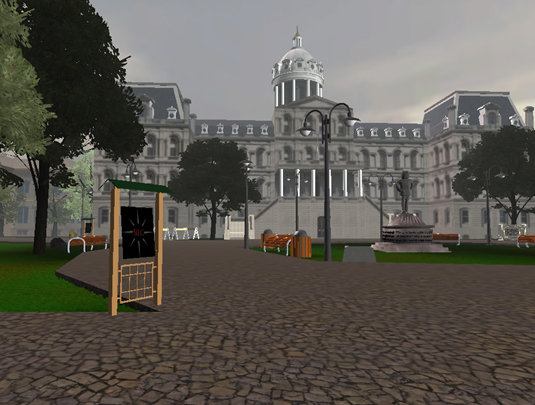
\includegraphics[width=12cm,height=6cm]{./figs/Cover_Page.jpg}\\[\bigskipamount]

\begin{figure}[!htb]
\minipage{0.32\textwidth}
  
\includegraphics[width=\linewidth]{./figs/Temple.jpg}
  \caption*{}\label{fig:awesome_image1}
\endminipage\hfill
\minipage{0.32\textwidth}
  
\includegraphics[width=\linewidth]{./figs/SILC.jpg}
  \caption*{}\label{fig:awesome_image2}
\endminipage\hfill
\minipage{0.32\textwidth}%
  \includegraphics[width=\linewidth]{./figs/SCANN_LAB.png}
  \caption*{}\label{fig:awesome_image3}
\endminipage
\end{figure}

\end{center}
}
\ifluatex
  \usepackage{selnolig}  % disable illegal ligatures
\fi
\usepackage[]{natbib}
\bibliographystyle{apalike}

\title{Virtual Silcton Documentation}
\author{Steven M. Weisberg, PhD}
\date{15 February, 2021}

\begin{document}
\maketitle

{
\hypersetup{linkcolor=}
\setcounter{tocdepth}{1}
\tableofcontents
}
\setstretch{1.5}
\hypertarget{part-introduction}{%
\part*{Introduction}\label{part-introduction}}
\addcontentsline{toc}{part}{Introduction}

\hypertarget{virtual-silcton-introduction}{%
\chapter{Virtual Silcton Introduction}\label{virtual-silcton-introduction}}

Welcome to the documentation for \textbf{Virtual Silcton}.

The Virtual Silcton environment was originally designed in \href{https://unity.com/}{Unity3D} by \href{https://www.vrschinazi.com/}{Victor Schinazi} and Drew Dara-Abrams. In 2012, Steven Weisberg began updating and maintaining the documentation and website for administration of the Virtual Silcton environment.

This documentation was drafted by \href{scannlab.psych.ufl.edu}{Steven M. Weisberg} and last edited on the date at the top of this page.

\begin{figure}
\centering
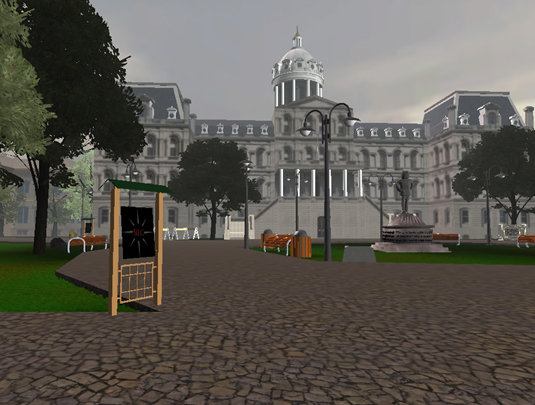
\includegraphics{./figs/Cover_Page.jpg}
\caption{Virtual Silcton Image}
\end{figure}

\hypertarget{important-links}{%
\section{Important Links}\label{important-links}}

\begin{enumerate}
\def\labelenumi{\arabic{enumi}.}
\tightlist
\item
  \href{www.virtualsilcton.com}{Virtual Silcton website}
\item
  \href{https://osf.io/fykr7/}{The Virtual Silcton standalone builds (Routes, Free Exploration, Onsite Pointing)}
\item
  \href{https://github.com/smweis/Virtual_Silcton_Analysis}{Virtual Silcton analysis code repo}
\item
  \href{https://github.com/Scann-Lab/VirtualSilctonUnity}{Virtual Silcton Unity files}
\end{enumerate}

The Virtual Silcton website is available for use. Please email \href{mailto:stevenweisberg@ufl.edu}{\nolinkurl{stevenweisberg@ufl.edu}} to setup an experimenter account and receive information about testing.

\hypertarget{virtual-silcton-background}{%
\chapter{Virtual Silcton Background}\label{virtual-silcton-background}}

Thank you for using the Vitual Silcton (\textbf{S}patial \textbf{I}ntelligence \and \textbf{L}earning \textbf{C}enter \textbf{T}est \textbf{o}f \textbf{N}avigation) navigation assessment. This documentation provides basic instructions, best practices, and documentation of experimental protocols and some data processing. The Virtual Silcton environment was initially developed by Victor R. Schinazi and Drew Dara-Abrams in a collaboration funded by the NSF as part of the Spatial Intelligence and Learning Center. Nora Newcombe and Russell Epstein spear-headed the initial project development until 2012, including developing the original 3D Unity files and placing the entire experiment on a website. Since 2012, Steven Weisberg has been responsible for maintaining and updating the Virtual Silcton platform. In 2019, the firm Gaia Solutions took over the web development side.

Virtual Silcton has been designed with the idea of creating a \emph{semi-customizable} but largely standard 3D virtual environment measure of navigation behavior. Silcton trades off flexibility for stability. Although not all experimental designs are possible, this means that most studies which use Silcton are comparable because all participants experience largely the same environment, in mostly the same order, and are assessed the same way.

\begin{figure}
\centering
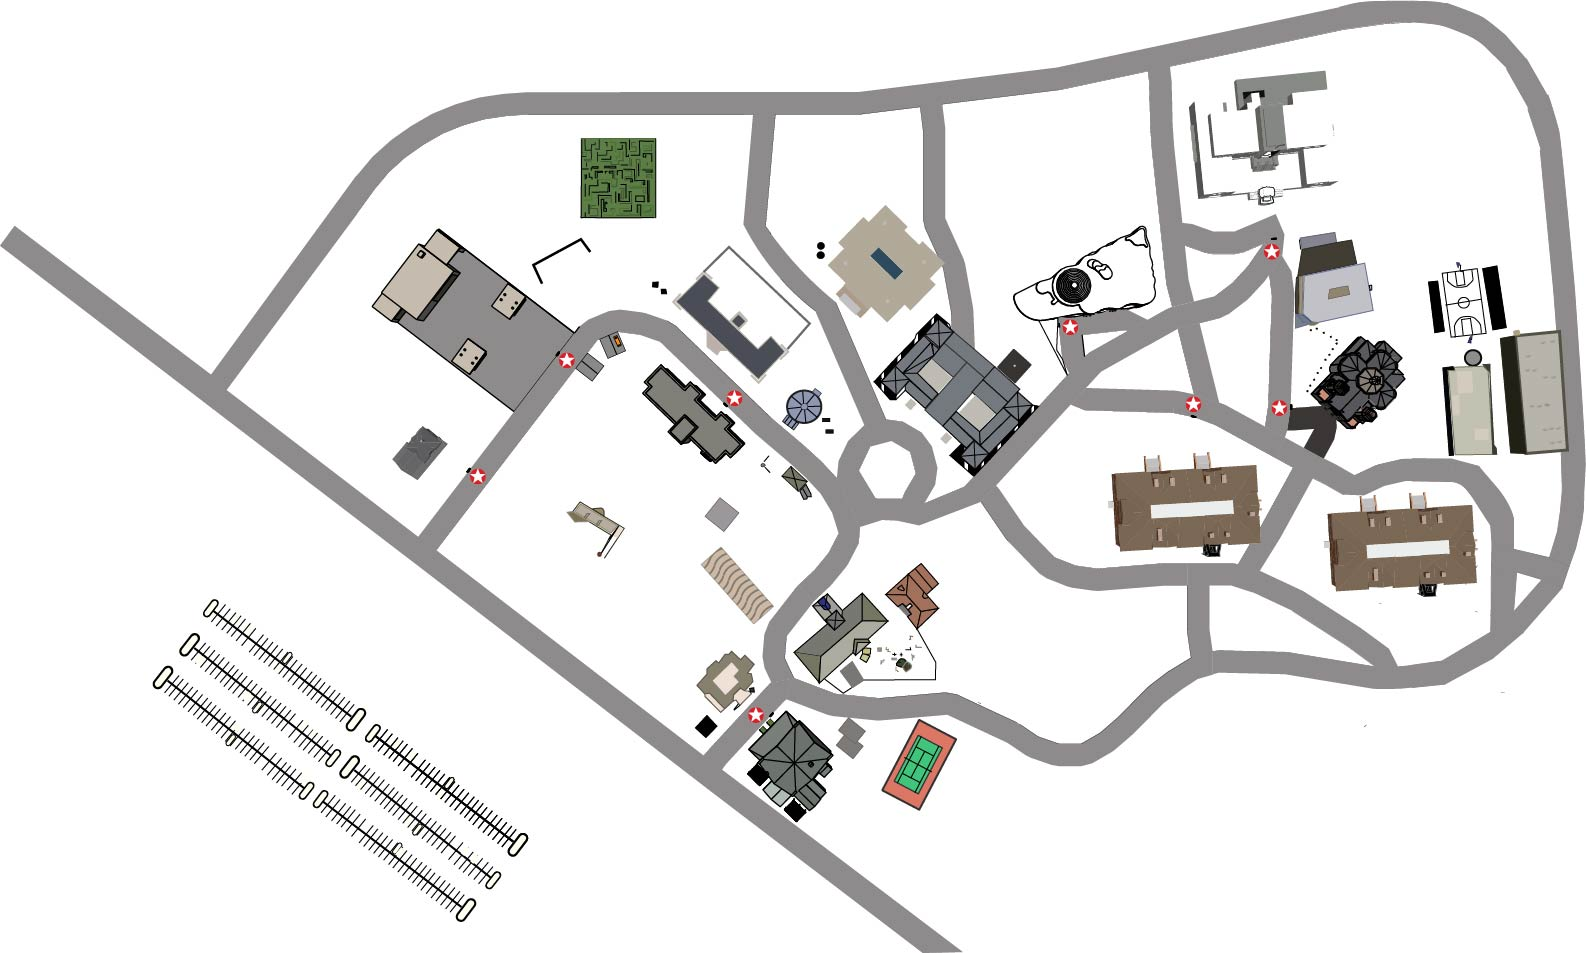
\includegraphics{./figs/Full_Info_Silcton_map_NoBG.jpg}
\caption{Virtual Silcton Map (Red lines highlight main routes)}
\end{figure}

\hypertarget{real-world-ambler-campus}{%
\section{Real World Ambler Campus}\label{real-world-ambler-campus}}

The Virtual Silcton environment is built as a virtual replica of Temple's Ambler campus outside Philadelphia, Pennsylvania. In that suburban college campus, Victor Schinazi and colleagues ran approximately 15 subjects through a real-world version of the Silcton experiment in three sessions. Among their findings, it was evident that subjects had wide variability for learning the environment successfully over time. It was time to scale up.

\hypertarget{virtual-silcton-studies}{%
\section{Virtual Silcton studies}\label{virtual-silcton-studies}}

The initial Virtual Silcton experiments were designed to measure individual differences in spatial navigation behavior objectively and see if individual variability could be correlated with other measures of cognitive traits. These experiments (including \href{https://psycnet.apa.org/fulltext/2013-44238-001.html}{Weisberg et al., 2013} and \href{https://psycnet.apa.org/fulltext/2015-52470-001.html}{Weisberg \& Newcombe (2016)}), revealed substantial variation in performance across people. Although performance on Silcton was correlated with a self-report measure of navigation behavior (the Santa Barbara Sense of Direction Scale), unique variance was explained by measures like the mental rotation test and working memory measures.

Beyond the initial experiments, a large number of labs and experimenters have used the Virtual Silcton software to measure individual differences in spatial navigation behavior.

\hypertarget{who-should-use-this}{%
\section{Who should use this?}\label{who-should-use-this}}

Are you interested in measuring variability in spatial navigation behavior quickly and cheaply, but wish to go beyond self-report? The Virtual Silcton website may be what you're looking for. Check out \protect\hyperlink{administering-to-participants}{Administering to Participants}.

\hypertarget{administering-to-participants}{%
\chapter{Administering to Participants}\label{administering-to-participants}}

Data collection can proceed through three main avenues, described in brief below.

\hypertarget{website-administration}{%
\section{Website Administration}\label{website-administration}}

If you wish to take full advantage of the Silcton measures, setting up a lab account with the Virtual Silcton website is the way to go.

You'll have access to the {[}Silcton{]}{[}\#Silcton Measures{]} and {[}Other{]}{[}\#Other Measures{]}; your data will be stored and accessible via the cloud; you'll be able to customize your studies (which partition your data); and you can run all studies online.

However, your data will be public (for participants who agree, after a maximum of 3 years upon beginning the study) and accessible to all other website users.

You also have limited customization options.

\hypertarget{standalone-builds}{%
\section{Standalone Builds}\label{standalone-builds}}

If you are concerned about data security, a stable internet connection, or want to have a non-internet backup for the study, we provide the following measures as standalone Unity builds:

\begin{itemize}
\tightlist
\item
  Main routes
\item
  Connecting routes
\item
  Free exploration
\item
  Onsite pointing task
\end{itemize}

See the OSF page for details: \url{https://osf.io/fykr7/}

Note: The navigation logs and onsite pointing data will automatically export to your /Documents folder (Windows) or your Home folder (Mac).

We also provide analysis code for the onsite pointing data on our Github page: \url{https://github.com/smweis/Virtual_Silcton_Analysis}

\hypertarget{unity-files}{%
\section{Unity Files}\label{unity-files}}

If you'd like something besides the encoding or retrieval measures we provide, we also have the Unity files available as a Github repository: \url{http://github.com/Scann-Lab/VirtualSilctonUnity/}

There are two branches:

\begin{itemize}
\tightlist
\item
  Master: The standard Unity scenes for the website and Standalone
\item
  SilctonViveVR: The Unity scenes for use with the HTC Vive VR headset and Virtuix Omnidirectional treadmill.
\end{itemize}

Our ability to provide support for using these files is extremely limited.

\hypertarget{canonical-silcton}{%
\section{Canonical Silcton}\label{canonical-silcton}}

The ``canonical Silcton'' setup is as follows:

\begin{itemize}
\tightlist
\item
  SBSOD
\item
  Virtual Silcton Route Learning (Main Routes)
\item
  Virtual Silcton Route Learning (Main Routes)
\item
  Virtual Silcton Route Learning (Connecting Routes)
\item
  Virtual Silcton Route Learning (Connecting Routes)
\item
  Onsite Pointing
\item
  Model building
\end{itemize}

\hypertarget{part-virtual-silcton-website}{%
\part{Virtual Silcton Website}\label{part-virtual-silcton-website}}

\hypertarget{experimenter-interface}{%
\chapter{Experimenter Interface}\label{experimenter-interface}}

If you are interested in collecting your own data using the Virtual Silcton \emph{website}, start here.

To begin, you need to set up an account. Email Steven Weisberg \href{mailto:stevenweisberg@ufl.edu}{stevenweisberg at ufl dot edu} using an institutional email and provide a current CV. You will receive instructions for how to login.

\hypertarget{a-note-about-irb-approval}{%
\section{A note about IRB Approval}\label{a-note-about-irb-approval}}

Temple University maintains an omnibus IRB protocol, which covers administrative access to the Virtual Silcton website. Steven Weisberg, Nora Newcombe, web developers in our employment will have access to data collected from all \emph{Labs}.

\emph{YOU MUST OBTAIN YOUR OWN INSTITUTE'S IRB APPROVAL}. To run your own study, you are required to provide informed consent at follow all protocols under a separate IRB from your home institution. Steven Weisberg and Nora Newcombe do not manage or maintain this information. \protect\hyperlink{consent}{See also Section 7.1}

\hypertarget{setting-up-an-account}{%
\section{Setting up an Account}\label{setting-up-an-account}}

The link you receive will send you to the Silcton Splash page:

\begin{figure}
\centering
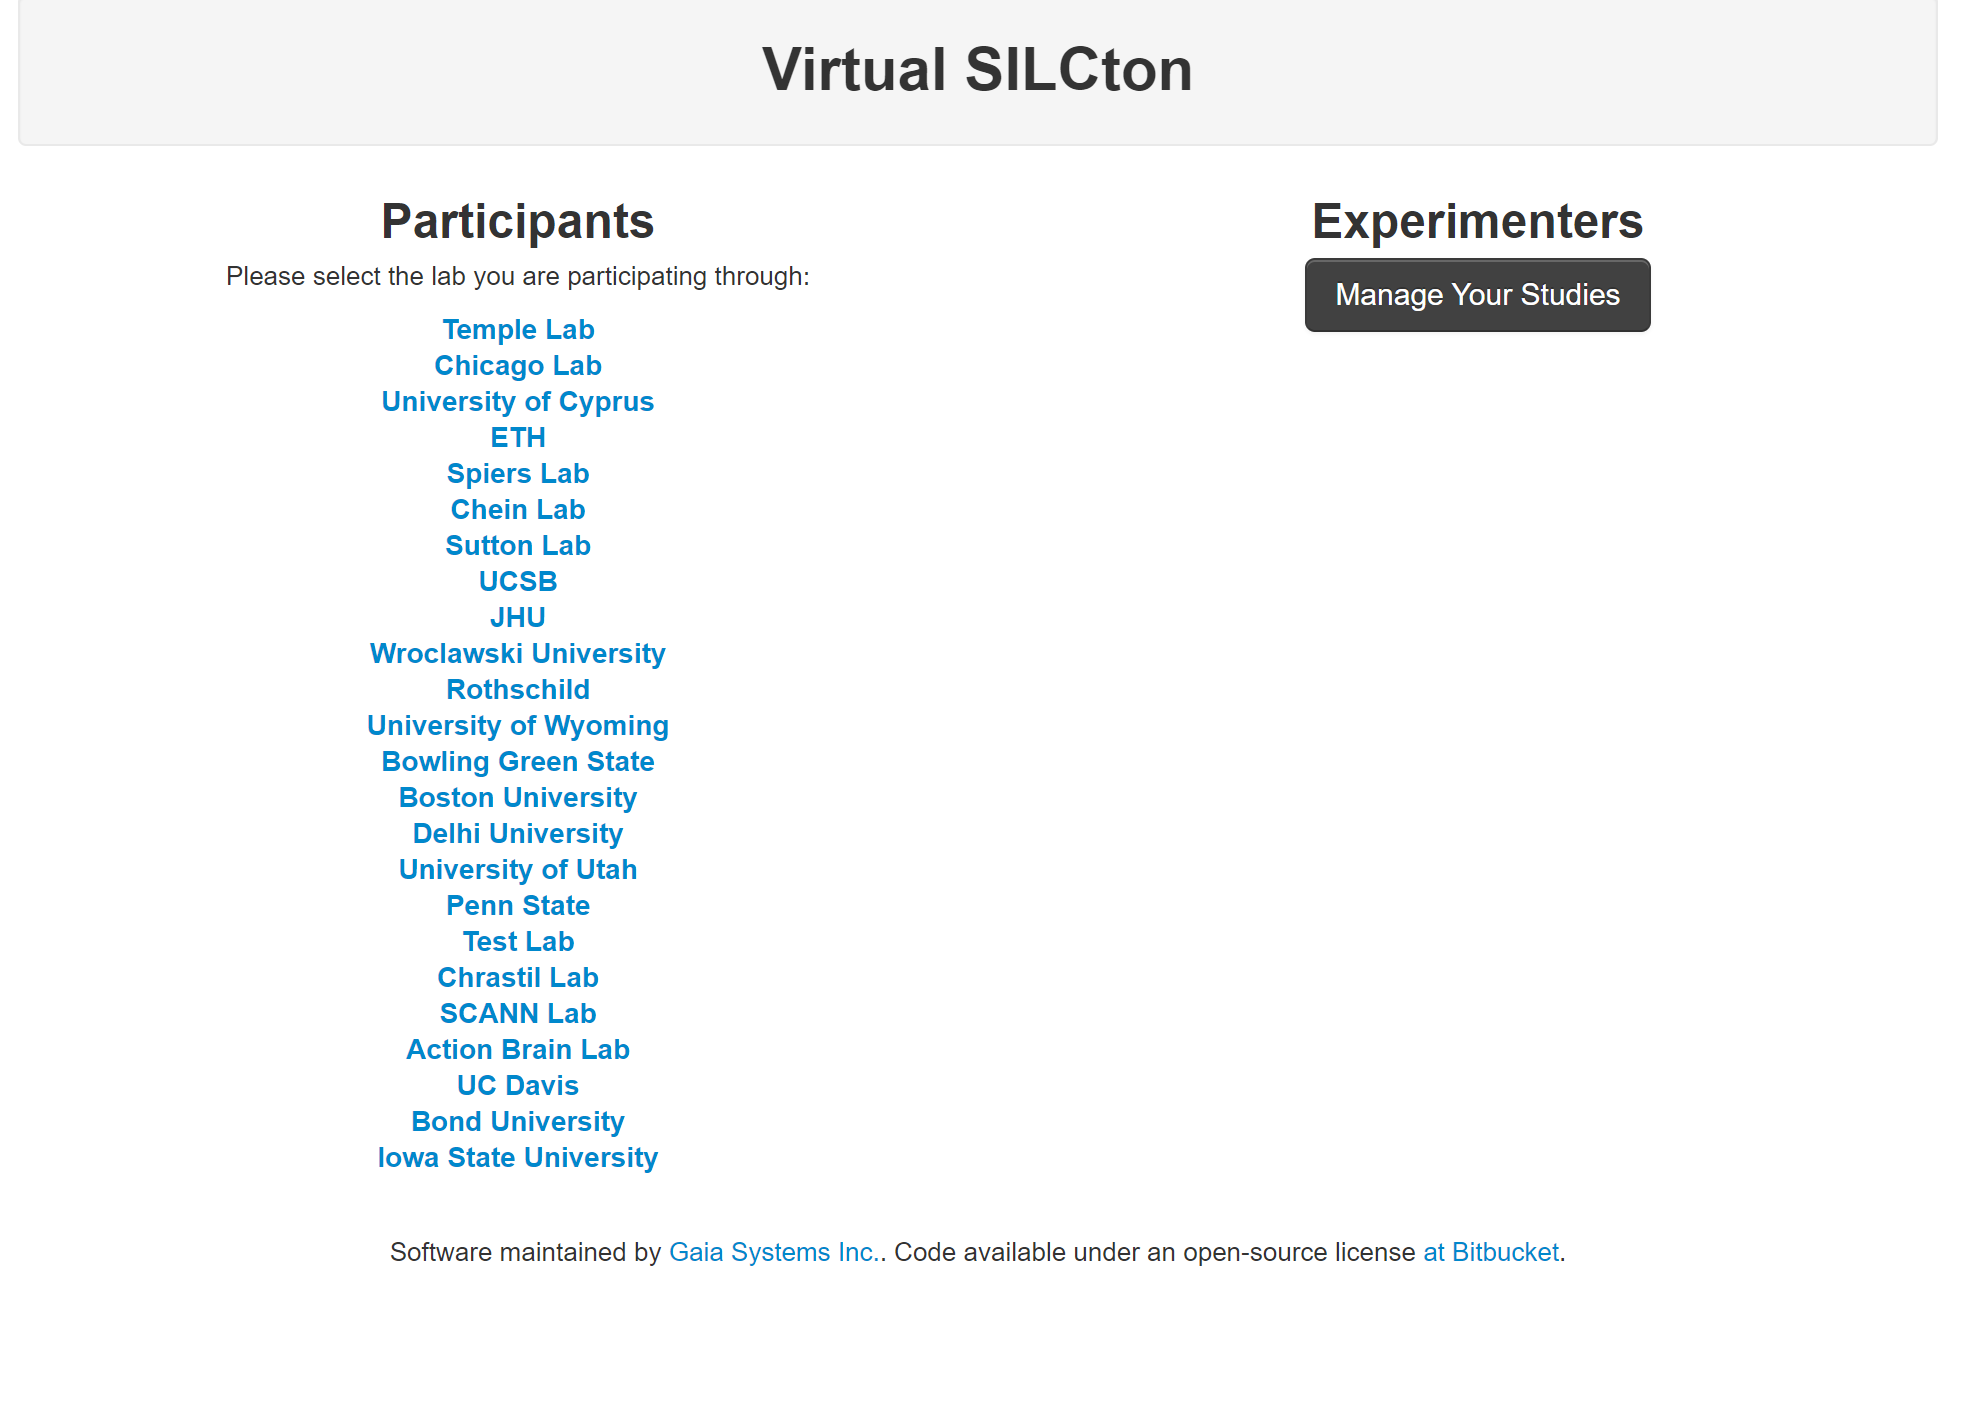
\includegraphics{./figs/exp_interface_1.png}
\caption{Virtual Silcton Splash Page}
\end{figure}

The links on the left will route participants to the studies that are visible on the website.

The link on the right, ``Manage Studies'', will take you to the experimenter interface. The administrator has created a \emph{Lab} for you, which you can log into.

The Virtual Silcton Website is broken up into \emph{Labs}, which are only accessible to Administrators (Steven Weisberg, Nora Newcombe, web developers) and Lab-specific personnel. In your lab, only the people whose accounts you set up will have access to your studies and data.

\hypertarget{labs}{%
\section{Labs}\label{labs}}

Labs are the main partition of the Virtual Silcton Website. Each \emph{Lab} has the capability of creating studies, administering studies, and managing their own data. No other labs have access to your data.

\hypertarget{studies}{%
\section{Studies}\label{studies}}

A Study is a data collection partition within a lab. All participants collected via one Study will be affiliated together throughout the Experimenter Interface. Studies can be customized in various ways (See \protect\hyperlink{building-studies}{Building Studies}.)

Clicking on the \emph{Studies} tab of the Experimenter Interface displays all Studies your lab has created, along with some meta-data about the Study.

\begin{figure}
\centering
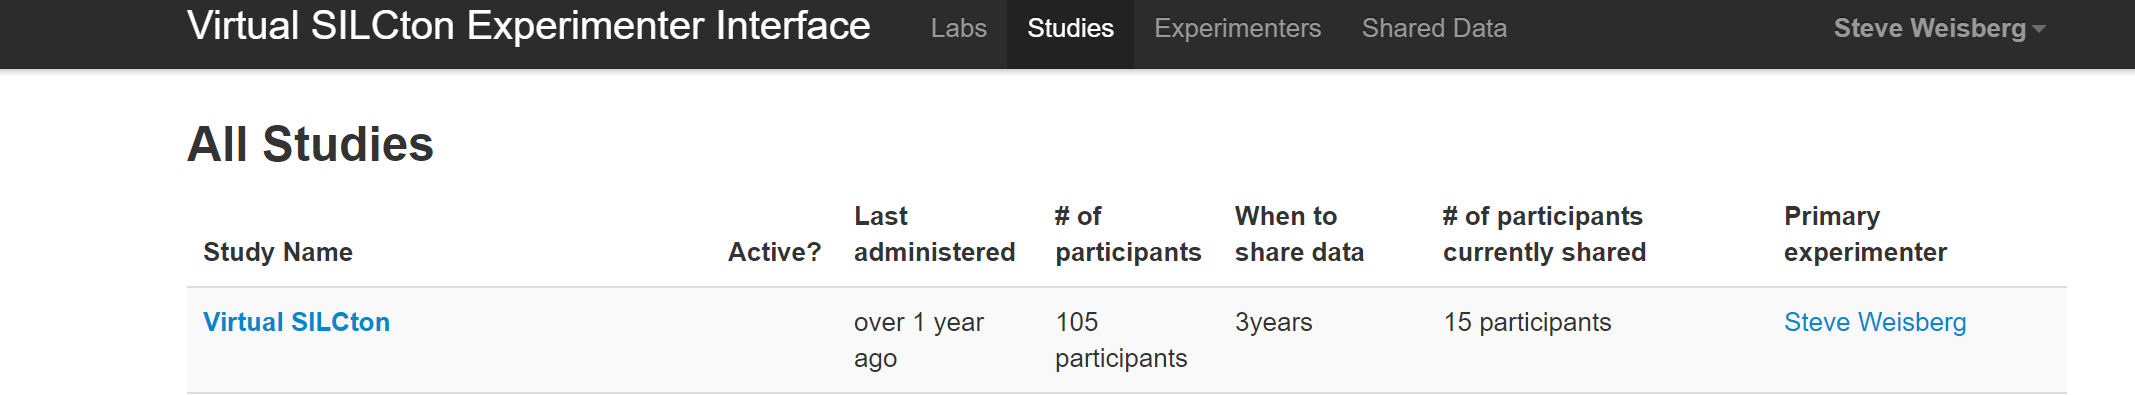
\includegraphics{./figs/exp_interface_2.png}
\caption{Virtual Silcton Studies}
\end{figure}

\hypertarget{account-types}{%
\section{Account Types}\label{account-types}}

\hypertarget{experimenters}{%
\subsection{Experimenters}\label{experimenters}}

For the lab they belong to:
1. Can view materials, participants, and data from the Experimenter Interface.
2. Can edit Studies and delete Participants for Studies which they have been assigned Primary Experimenter.

For all labs:
3. View publicly-available data. (See \protect\hyperlink{building-studies}{Studies}).

\hypertarget{lab-managers}{%
\subsection{Lab Managers}\label{lab-managers}}

Have all the capabilities of Experimenters, PLUS:
For the lab they belong to:
1. Can delete participants.
2. Can view all lab data.
3. Can add, edit, and delete Lab Managers, Experimenters, and Studies.

\hypertarget{administrators}{%
\subsection{Administrators}\label{administrators}}

Have all the capabilities of Lab Managers, PLUS:
For all labs:
1. Can delete participants.
2. Can add, edit, and delete Studies.
3. Can add, edit, and delete Administrators.

\hypertarget{building-studies}{%
\chapter{Building Studies}\label{building-studies}}

\hypertarget{create-study}{%
\section{Create Study}\label{create-study}}

In the Study tab of the Experimenter Interface, you can view all Studies you created along with their meta-data. Scrolling to the bottom of this list, you'll find a ``Create Study'' button. Clicking this will create a new Study.

\hypertarget{edit-study}{%
\section{Edit Study}\label{edit-study}}

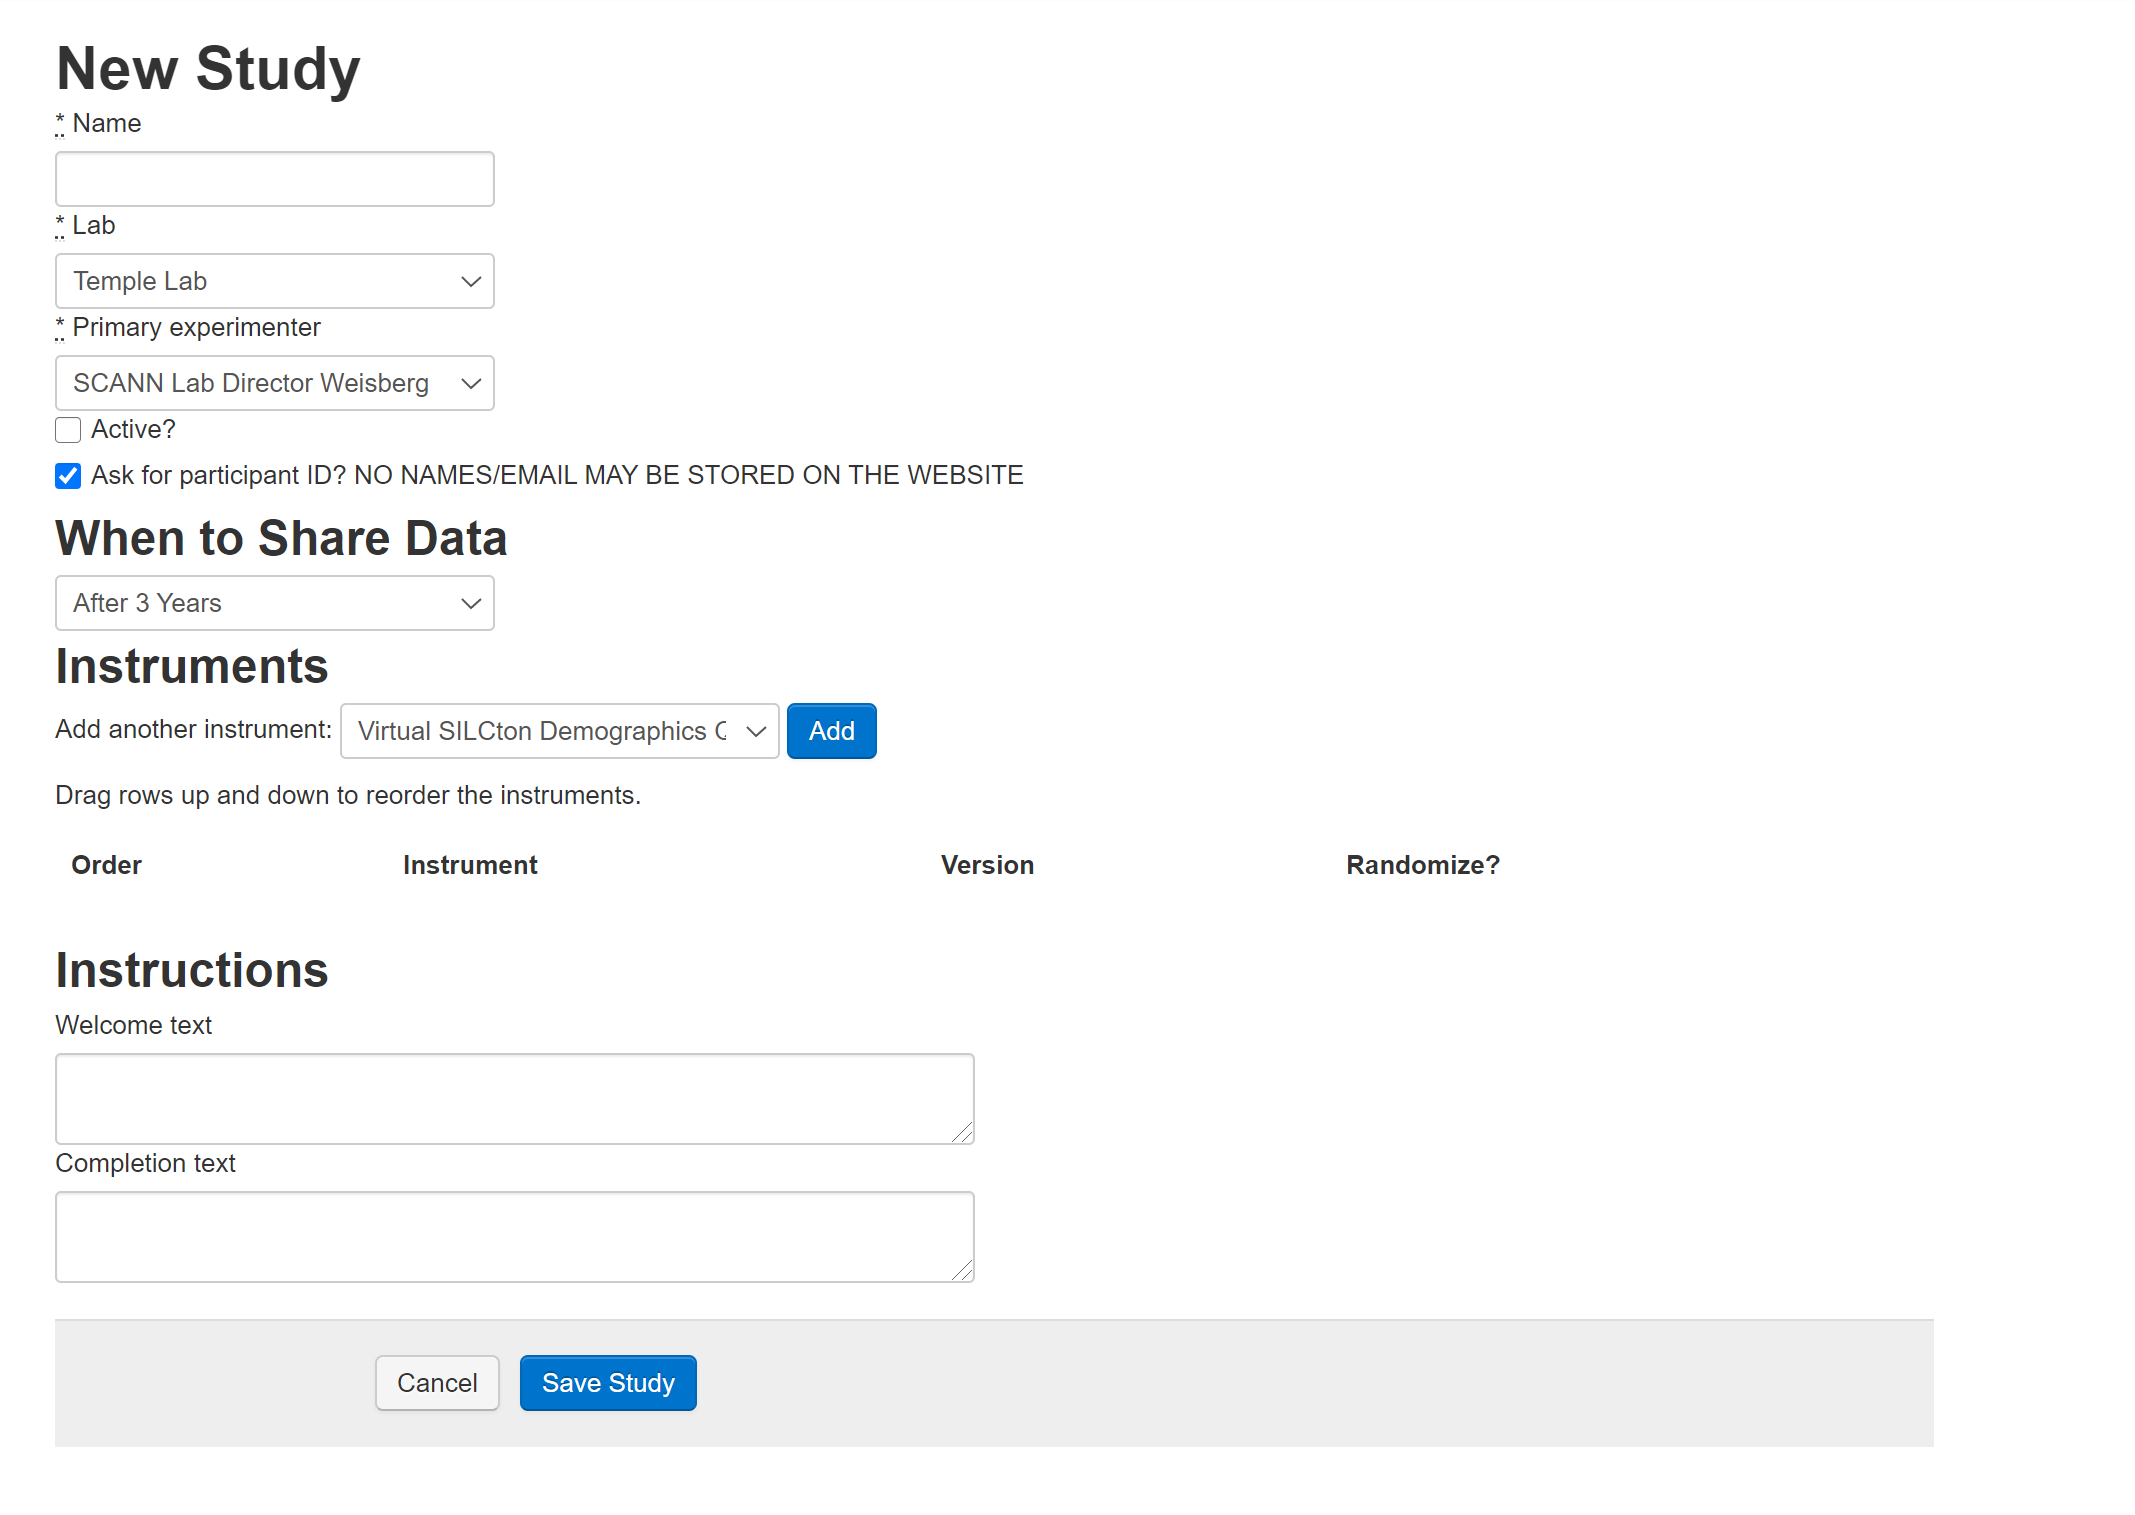
\includegraphics{./figs/web_studies_1.png}
When you first create a study (or, if you click ``Edit Study'' for a study you've already created), you will be able to customize it with the following options:

\begin{enumerate}
\def\labelenumi{\arabic{enumi}.}
\tightlist
\item
  Name: How your study will be referenced throughout the Silcton website.
\item
  Lab: The lab the study is affiliated with. (Note, if you choose a lab you are not affiliated with, you will not have access to the data collected from it.)
\item
  Primary Experimenter: The experimenter in charge of editing the study. (Note, Lab Managers will still be able to edit participants and studies for their lab. If an Experimenter is assigned this role, they will have these capabilities only for this Study).
\item
  Active: If checked, the Study will be viewable by any visitor to the main web page. \textbf{ONLY CHECK THIS FOR STUDIES YOU HAVE IRB APPROVAL TO RECRUIT AND COLLECT DATA FOR ANYONE WHO FINDS THE WEBSITE}
\item
  Ask for participant ID? (DEPRECATED - no custom IDs are possible.)
\item
  When to Share Data: All data collected via the Virtual Silcton repository will be made public after a 3-year embargo period for Participants who agree to the Web Data Release. The experimenter has the option to make data public immediately rather than waiting 3-years. Public data are made available to all Virtual Silcton website users.
\item
  Instruments: The dropdown menu provides all instruments available through Virtual Silcton. See \protect\hyperlink{silcton-measures}{Silcton Measures} and {[}Other Measures{]}. Instruments can be added in any combination (including repetitions) to Studies. To add an Instrument, navigate to the Edit Study view for the study you wish to edit, select the Instrument from the dropdown menu, and click ``Add.'' Once added to the list, Instruments can be dragged-and-dropped to any order you wish.
\item
  Welcome Text: Text entered here will appear on the first page the participant sees. (HTML Tags can be used in this field.)
\item
  Completion Text: Text entered here will appear after the final instrument is completed. (HTML Tags can be used in this field.)
\end{enumerate}

Once the study has been created, click Save Study.

After you save the Study, you'll see 4 tabs.

\begin{figure}
\centering
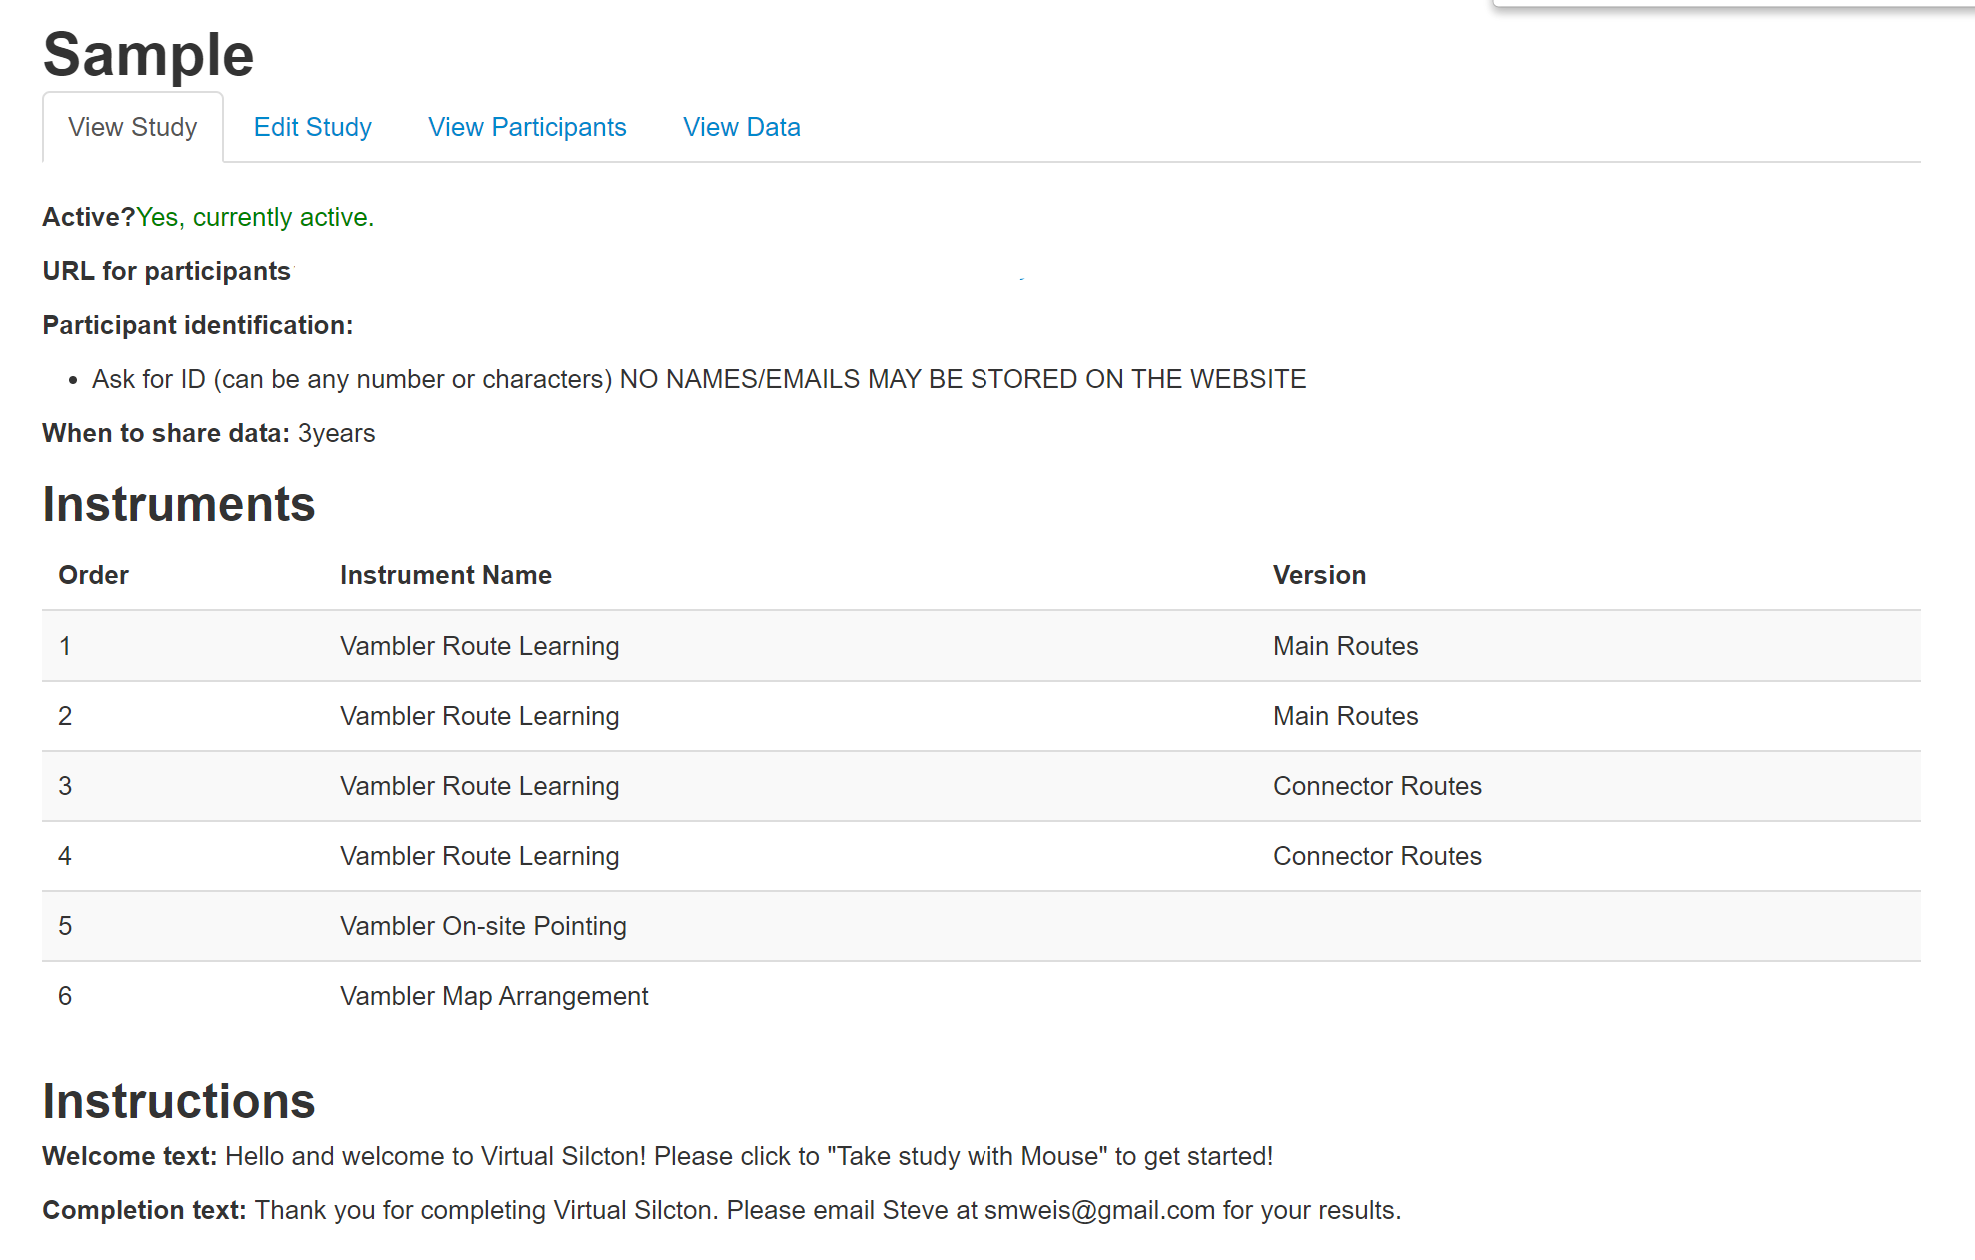
\includegraphics{./figs/web_studies_2.png}
\caption{Created Study View}
\end{figure}

View Study will show you the Study details.

Edit Study will allow you to edit the Study as you did when you created it.

View Participants will show you the Participants you collected thus far, their IDs, whether they've elected to share data, if they were designated a Pilot subject, and the date of data collection. You also have the option to Delete them, but \textbf{this action is not undoable} so use caution.

\begin{figure}
\centering
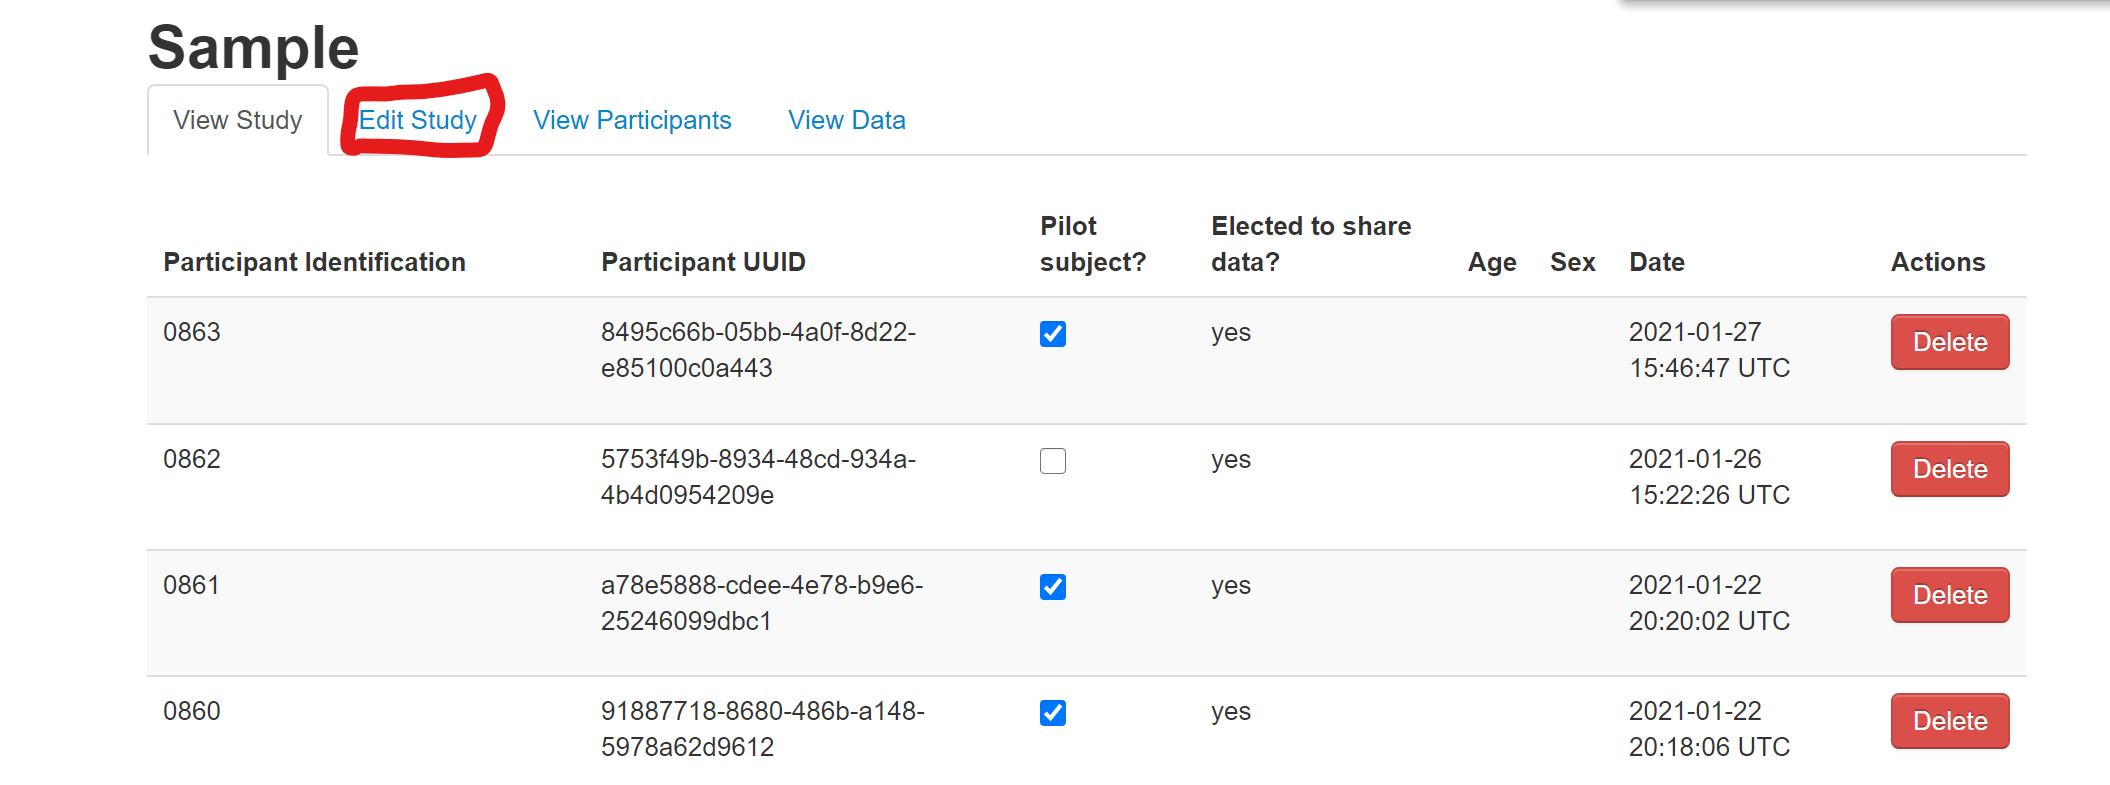
\includegraphics{./figs/web_studies_3.png}
\caption{View Participants}
\end{figure}

\hypertarget{participant-ids}{%
\subsection{Participant IDs}\label{participant-ids}}

Participants automatically receive two forms of ID in the Virtual Silcton study. A Participant UUID is a unique identifier assigned to every participant (whether supervised by an experimenter or not) who navigates to the Study Intro page (see {[}Other Measures{]}) and clicks Begin Experiment.

The UUID is random and unique, but not very user friendly.

A Participant Identification number will also be assigned once the experiment has begun. This number will increment by 1 for all data that was COLLECTED for that study.

In other words, if you collect Participant \#100, delete that participant, and run another participant, the second participant's number will be \#101.

\hypertarget{view-data}{%
\section{View Data}\label{view-data}}

\begin{figure}
\centering
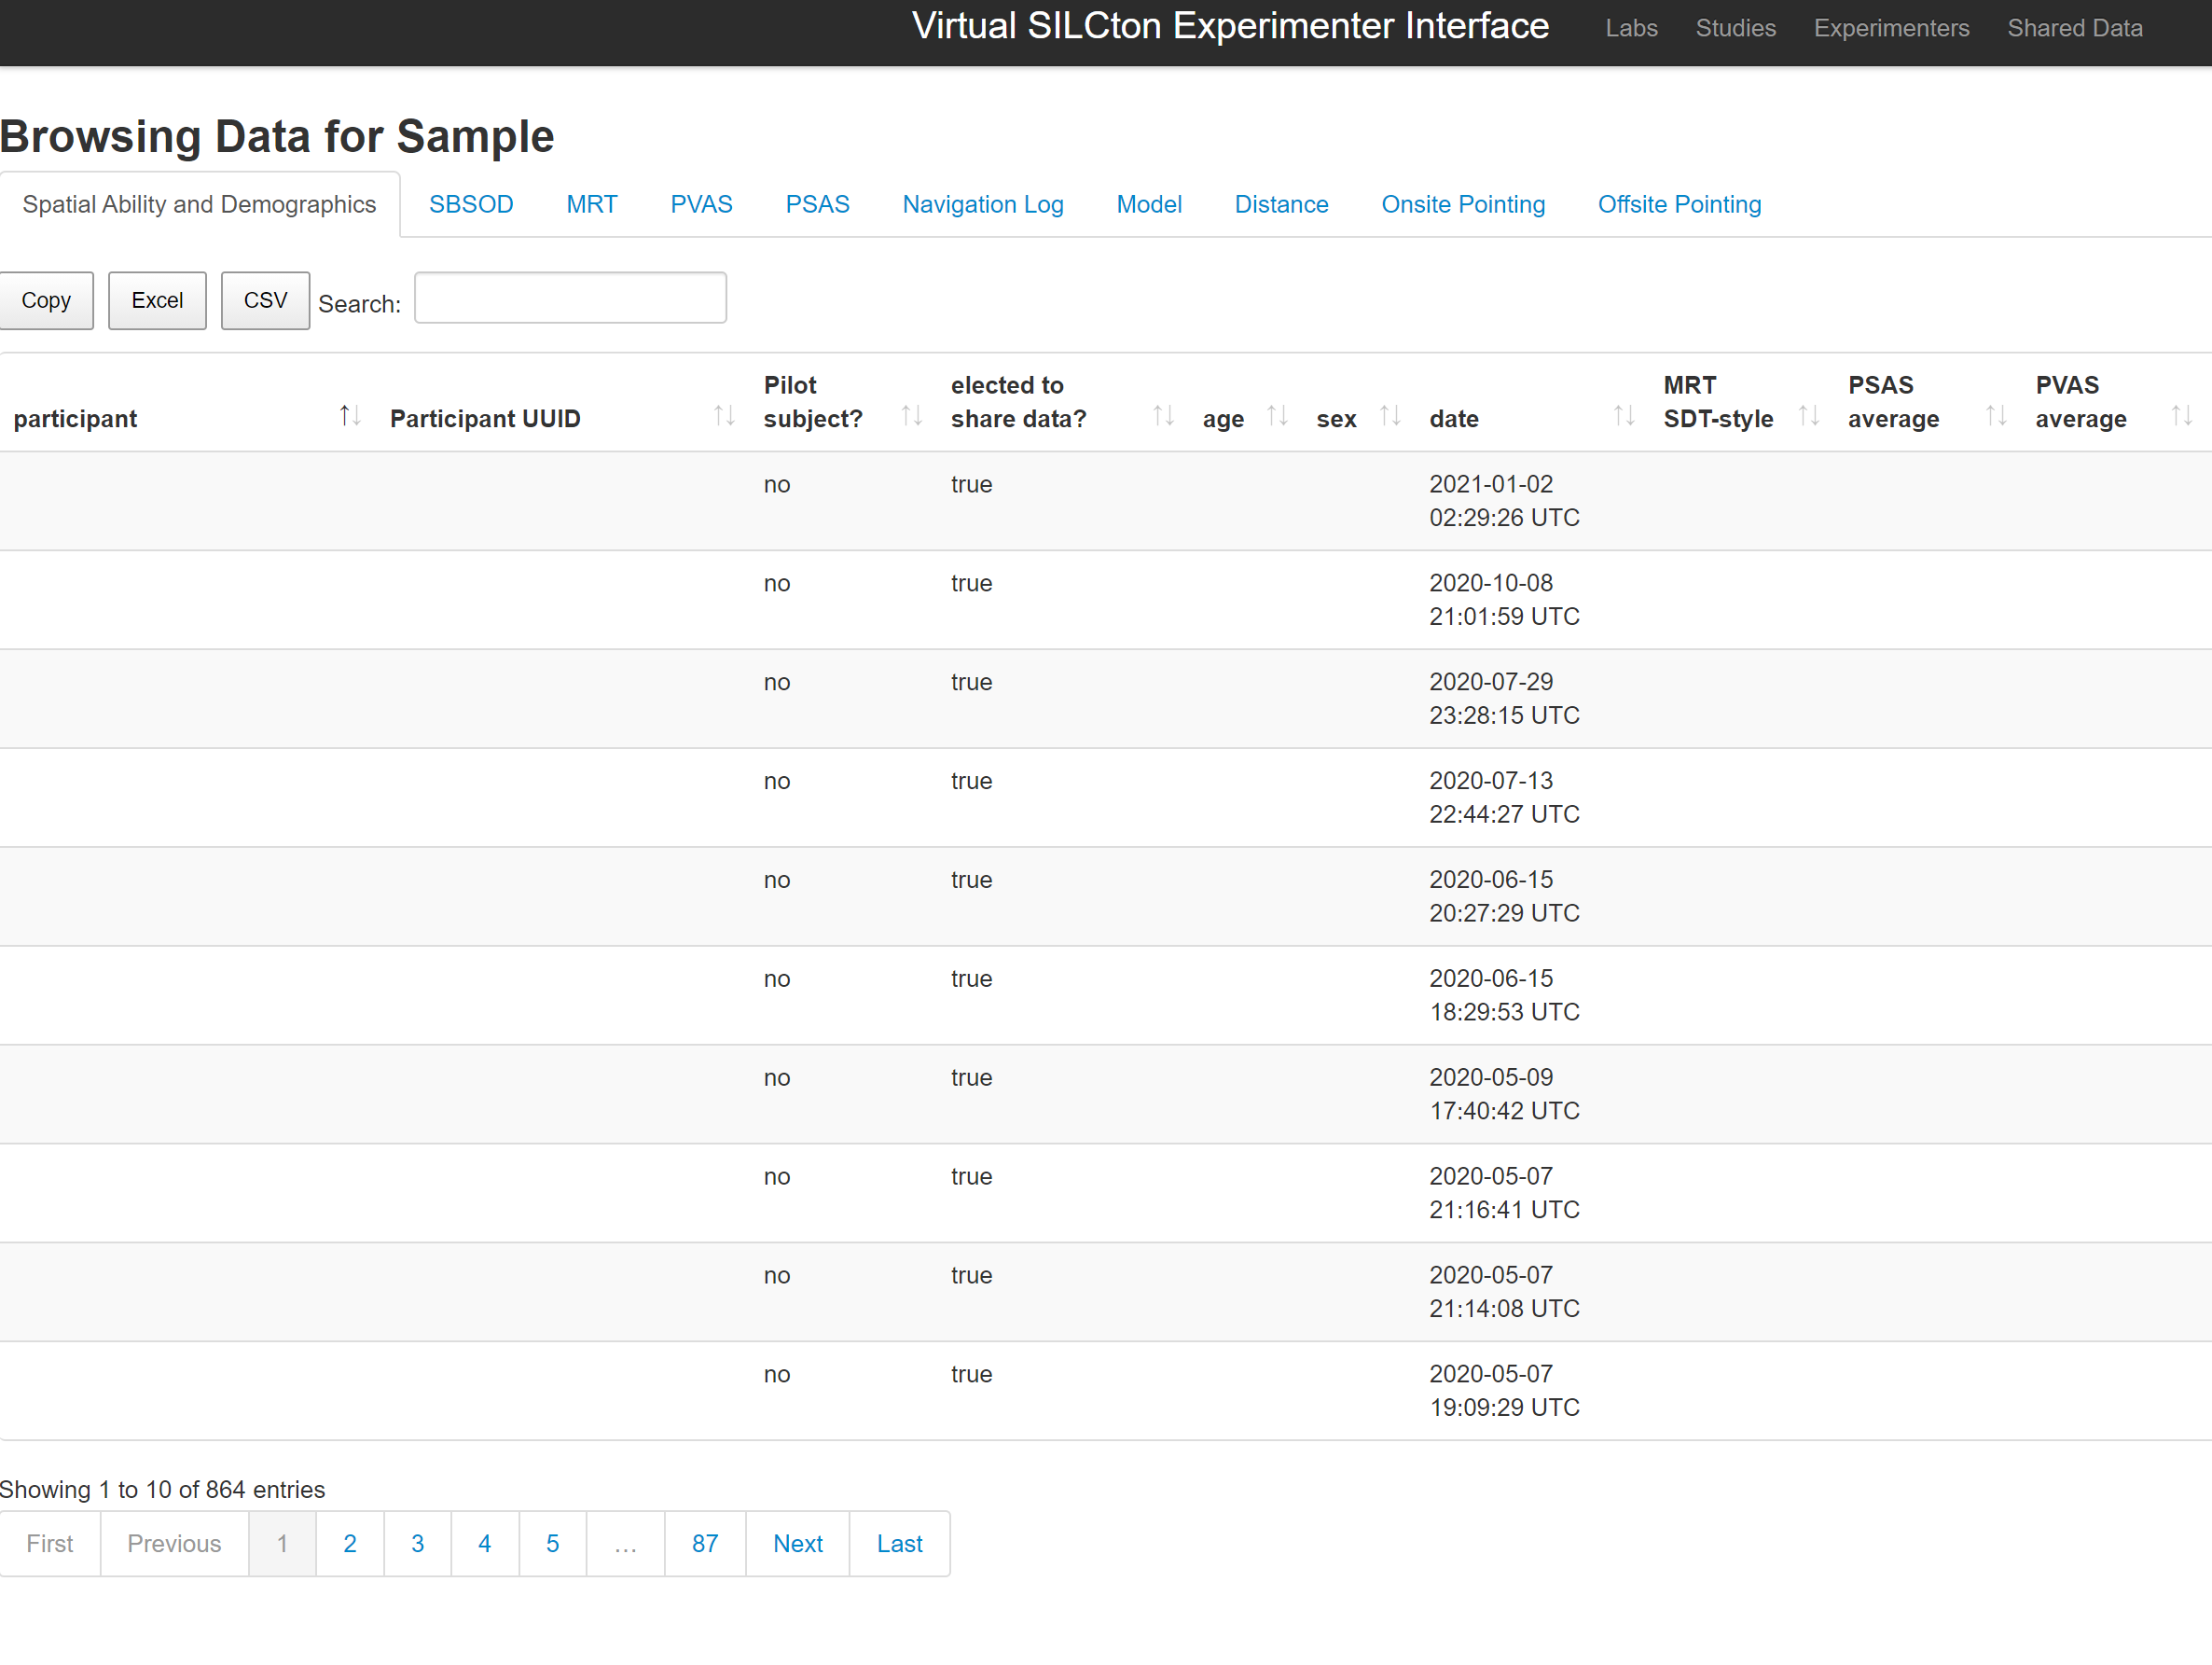
\includegraphics{./figs/web_studies_4.png}
\caption{View Data}
\end{figure}

The data for Virtual Silcton is split up across the various measures. The View Data tab allows you to view and download the data for each study. Unfortunately, this can only be done per measure at the moment.

Clicking {[}Copy{]}, {[}Excel{]}, {[}CSV{]} will save the data in those formats. For more information, see \protect\hyperlink{silcton-measures}{Silcton Measures} and {[}Other Measures{]}.

\hypertarget{interface-bugs}{%
\section{Interface Bugs}\label{interface-bugs}}

A quick note about the interface: It's a little clunky to move from the Study view to the Data view. In particular, the ``View Study'' button becomes highlighted during ``Edit Study.'' The easiest way to navigate from Data to Study views is to click back on Studies on the top black bar.

\hypertarget{silcton-measures}{%
\chapter{Silcton Measures}\label{silcton-measures}}

Virtual Silcton measures are those relating to the encoding and retrieval of the Silcton environment.

A note about online administration: load times may be long for the virtual environments. A relatively new computer, a stable internet connection, a recent version of Chrome or Firefox, and a traditional mouse (rather than a touchpad) are all recommended.

It is also recommended for all Virtual Silcton measures (except Distance and Offsite Pointing) that the Participant clicks the Blue arrows in the lower right of the screen to make it Full Screen.

The Encoding measures can be exited by pressing Escape on the keyboard, then clicking the ``I am Finished'' button that appears on the browser in the lower left.

The Onsite Pointing measure must be completed by clicking through all trials (56 in total).

\textbf{A note on landmark names:}
The landmarks names for Virtual Silcton were chosen to be distinctive and consistent with the building they name (e.g., a Museum-like building).

The names were also chosen in deference to notable geographers. In addition to being less than representative (all names belong to white men), in one case, this resulted in a gas station being named after a famous geographer, Kevin Lynch. We have adapted all materials to participants to clarify that all buildings were named in such a manner, and recommend that all experimenters notify their participants as well.

\begin{itemize}
\item
  \href{https://en.wikipedia.org/wiki/Michael_Batty}{Michael Batty}
\item
  \href{https://en.wikipedia.org/wiki/Kevin_A._Lynch}{Kevin Lynch}
\item
  \href{https://en.wikipedia.org/wiki/Chauncy_Harris}{Chauncy Harris}
\item
  \href{https://en.wikipedia.org/wiki/David_Harvey}{David Harvey}
\item
  \href{https://en.wikipedia.org/wiki/Reginald_Golledge}{Reginald Golledge}
\item
  \href{https://en.wikipedia.org/wiki/John_Snow}{John Snow}
\item
  \href{https://en.wikipedia.org/wiki/Carl_O._Sauer}{Carl Sauer}
\item
  \href{https://en.wikipedia.org/wiki/Waldo_R._Tobler}{Waldo Tobler}
\end{itemize}

\hypertarget{encoding}{%
\section{Encoding}\label{encoding}}

All methods of encoding also record the Participant's facing direction and location every 100ms. These data can be found under the Navigation Log section of View Data.

\hypertarget{routes}{%
\subsection{Routes}\label{routes}}

Routes are prescribed paths through Virtual Silcton consisting of marked roads (using red arrows). Participants are bound along these routes by invisible walls that will prevent them from exploring beyond the routes.

\hypertarget{main-routes}{%
\subsubsection{Main Routes}\label{main-routes}}

The Main Routes (A and B) each consist of 4 named landmarks that the participant is responsible for learning. The landmarks are indicated along the route with a blue gem, and named with a yellow and red sign. It is suggested that the Participant navigate from the beginning of each main route to the end and back.

\begin{figure}
\centering
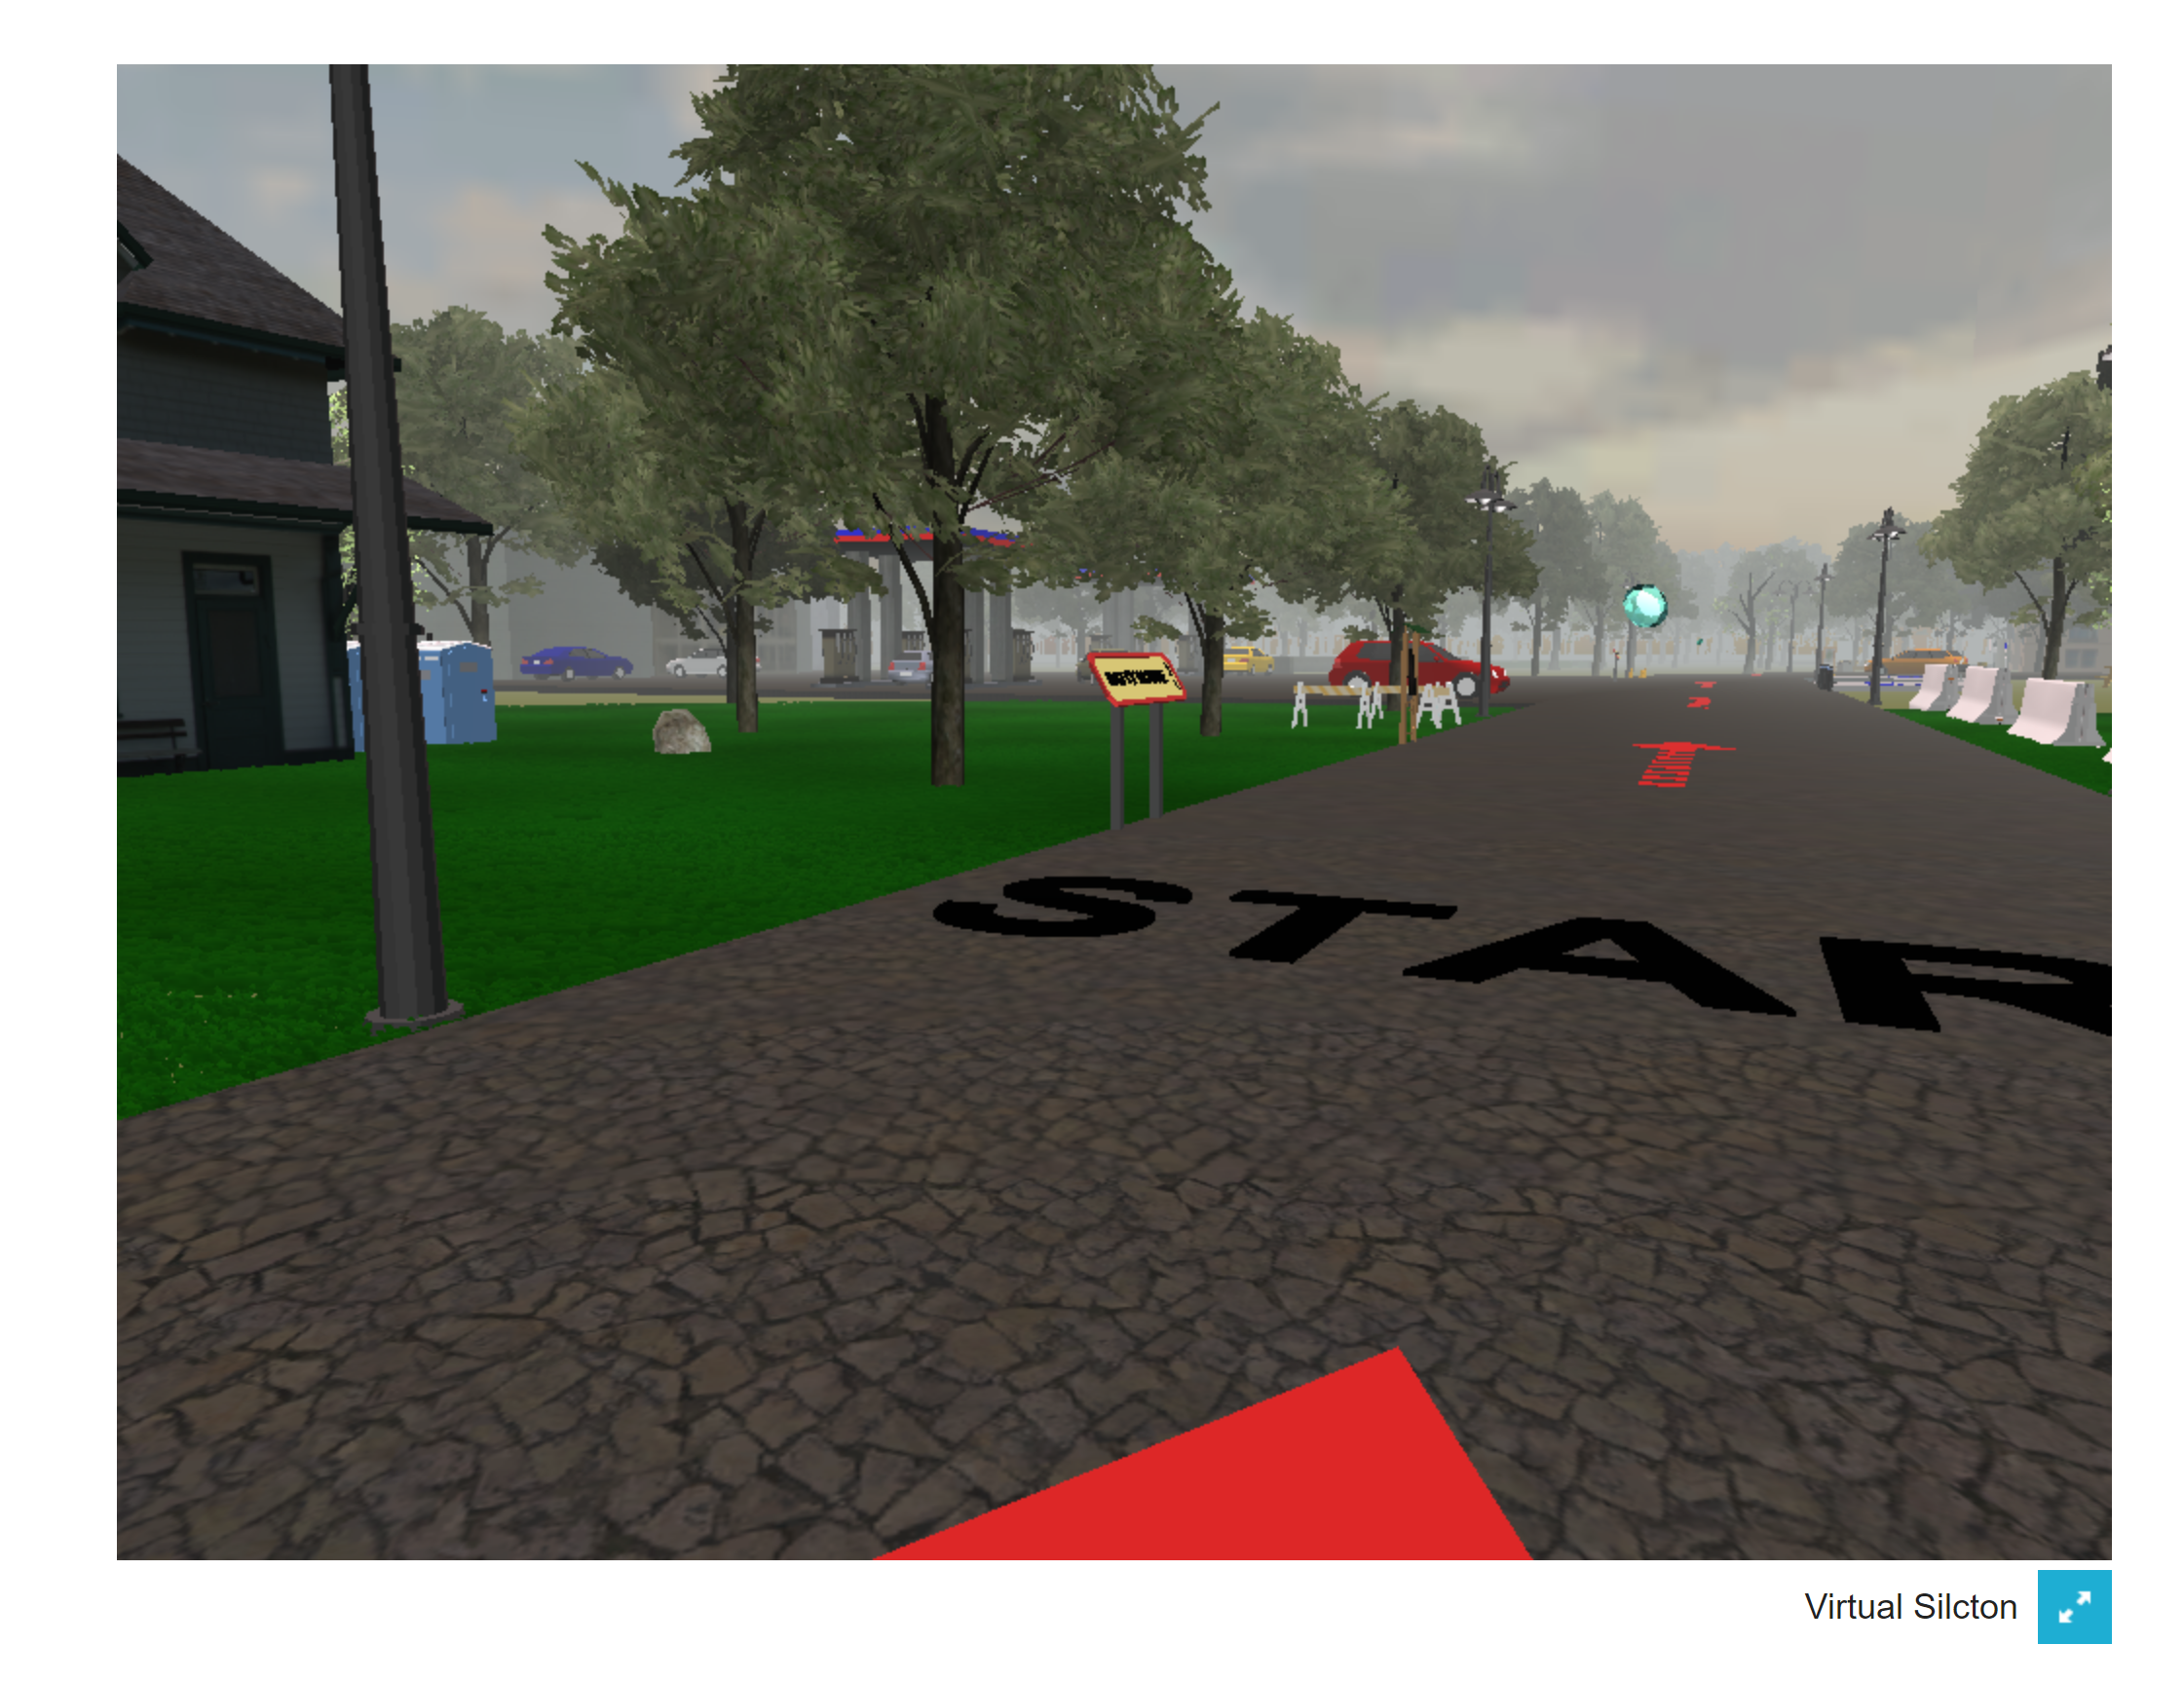
\includegraphics{./figs/Route_A.png}
\caption{Virtual Silcton Main Route A}
\end{figure}

\hypertarget{connecting-routes}{%
\subsubsection{Connecting Routes}\label{connecting-routes}}

The Connecting Routes (C1 and C2) are additional chances to explore the environment. Each Connecting Route connects one Main Route to the other. It is suggested that the participant navigate from the beginning of each Connecting Route to the end and back.

\hypertarget{fixed-vs.-random-route-presentation}{%
\subsubsection{Fixed vs.~Random Route Presentation}\label{fixed-vs.-random-route-presentation}}

In the Edit Study view, Main Routes and Connecting Routes can be added in a RANDOMIZED order or in a FIXED order.

For the standard Virtual Silcton learning paradigm, it is recommended to begin with both Main Routes (order randomized across Participants), followed by both Connecting Routes (order randomized across Participants).

To accomplish this, add the ``Virtual Silcton Route Learning (Main Routes)'' TWICE. Followed by the ``Virtual Silcton Route Learning (Connecting Routes)'' TWICE. This will randomize the order of the Main Routes and Connecting Routes across Participants.

However, you can also add as many presentations of each of the four routes in any order you wish. To do this, simply add the Instrument with the Route name: ``Virtual Silcton Route Learning (Main Route A)''. This will always present that route in that order. In other words, an Instrument ordering like this:

Virtual Silcton Route Learning (Main Route A)
Virtual Silcton Route Learning (Main Route B)
Virtual Silcton Route Learning (Main Route A)
Virtual Silcton Route Learning (Main Route C1)

Will present: A, B, A, C1.

Whereas this:
Virtual Silcton Route Learning (Main Routes)
Virtual Silcton Route Learning (Main Routes)
Virtual Silcton Route Learning (Connecting Routes)
Virtual Silcton Route Learning (Connecting Routes)

Will present: A/B, B/A, C1/C2, C2/C1.

\hypertarget{free-exploration-mode}{%
\subsection{Free Exploration Mode}\label{free-exploration-mode}}

In contrast to Routes, encoding can take place by the Participant wandering (or following directions provided by the experimenter) around the Virtual Silcton environment freely. Landmarks are still named, but there are no red arrows, nor are there invisible boundaries.

At this time, only one starting location is provided.

\hypertarget{retrieval}{%
\section{Retrieval}\label{retrieval}}

There are four retrieval tasks available at this time. Data can be downloaded for each separately through the View Data screen in the Experimenter Interface.

\hypertarget{onsite-pointing-task}{%
\subsection{Onsite Pointing Task}\label{onsite-pointing-task}}

The Onsite Pointing Task places the Participant next to each of the eight main landmarks, in the same fixed order (starting from the first building on Route A, through the last building on Route B). The Participant must point a crosshair in the center of the screen to the front door of the named building and click the mouse to indicate their response. Once they click, the prompt at the top of the screen will change. After the Participant has pointed to each landmark from the landmark they are standing next to (besides \emph{that} landmark), they will be placed next to the next landmark, where they will point to all the other landmarks again.

\begin{figure}
\centering
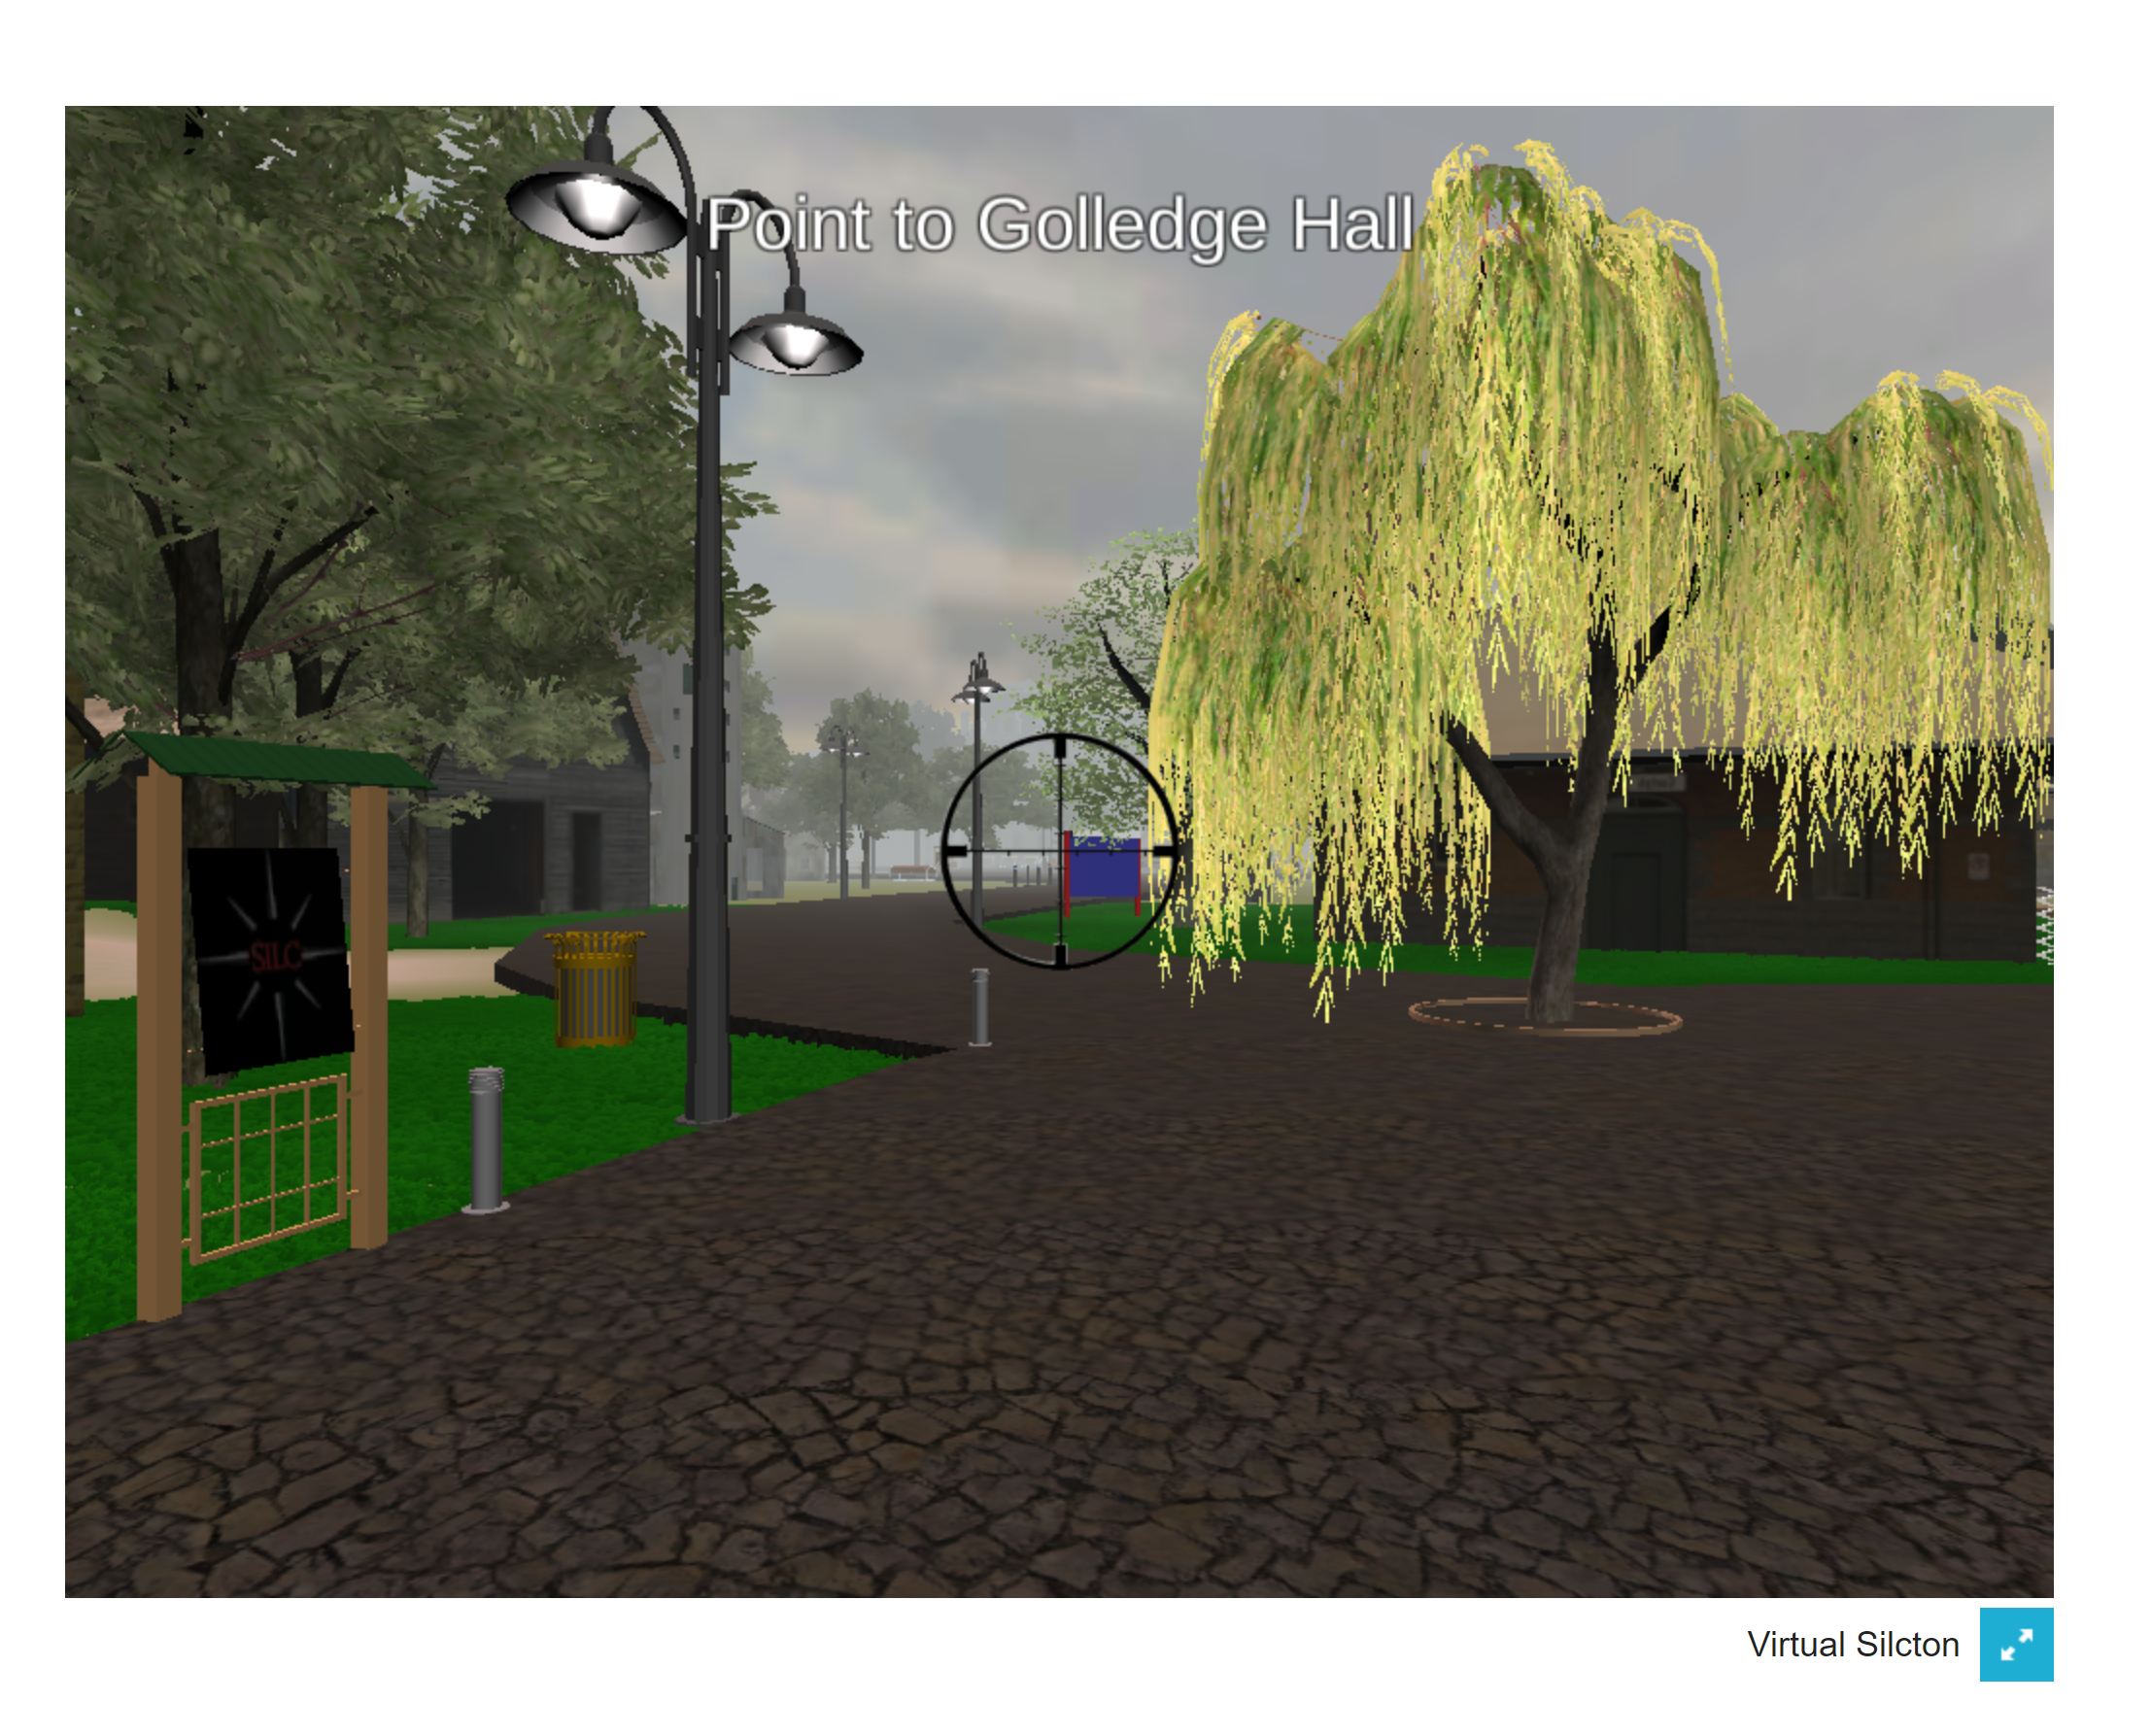
\includegraphics{./figs/Onsite_Pointing.png}
\caption{Virtual Silcton Onsite Pointing}
\end{figure}

\hypertarget{model-building-task}{%
\subsection{Model Building Task}\label{model-building-task}}

The model building task requires the Participant to drag and drop an aerial view image of each landmark to the position in the black outlined box that the Participant believes the landmark to be located.

Hovering over the aerial view image of each building displays a picture of the front view of the building along with its name.

Landmark models should be positioned FULLY INSIDE the black rectangle, or their positions may not be recorded.

Note: It is not possible to rotate the landmark models. This information can either be used by the Participant to aid them or can be ignored.

\begin{figure}
\centering
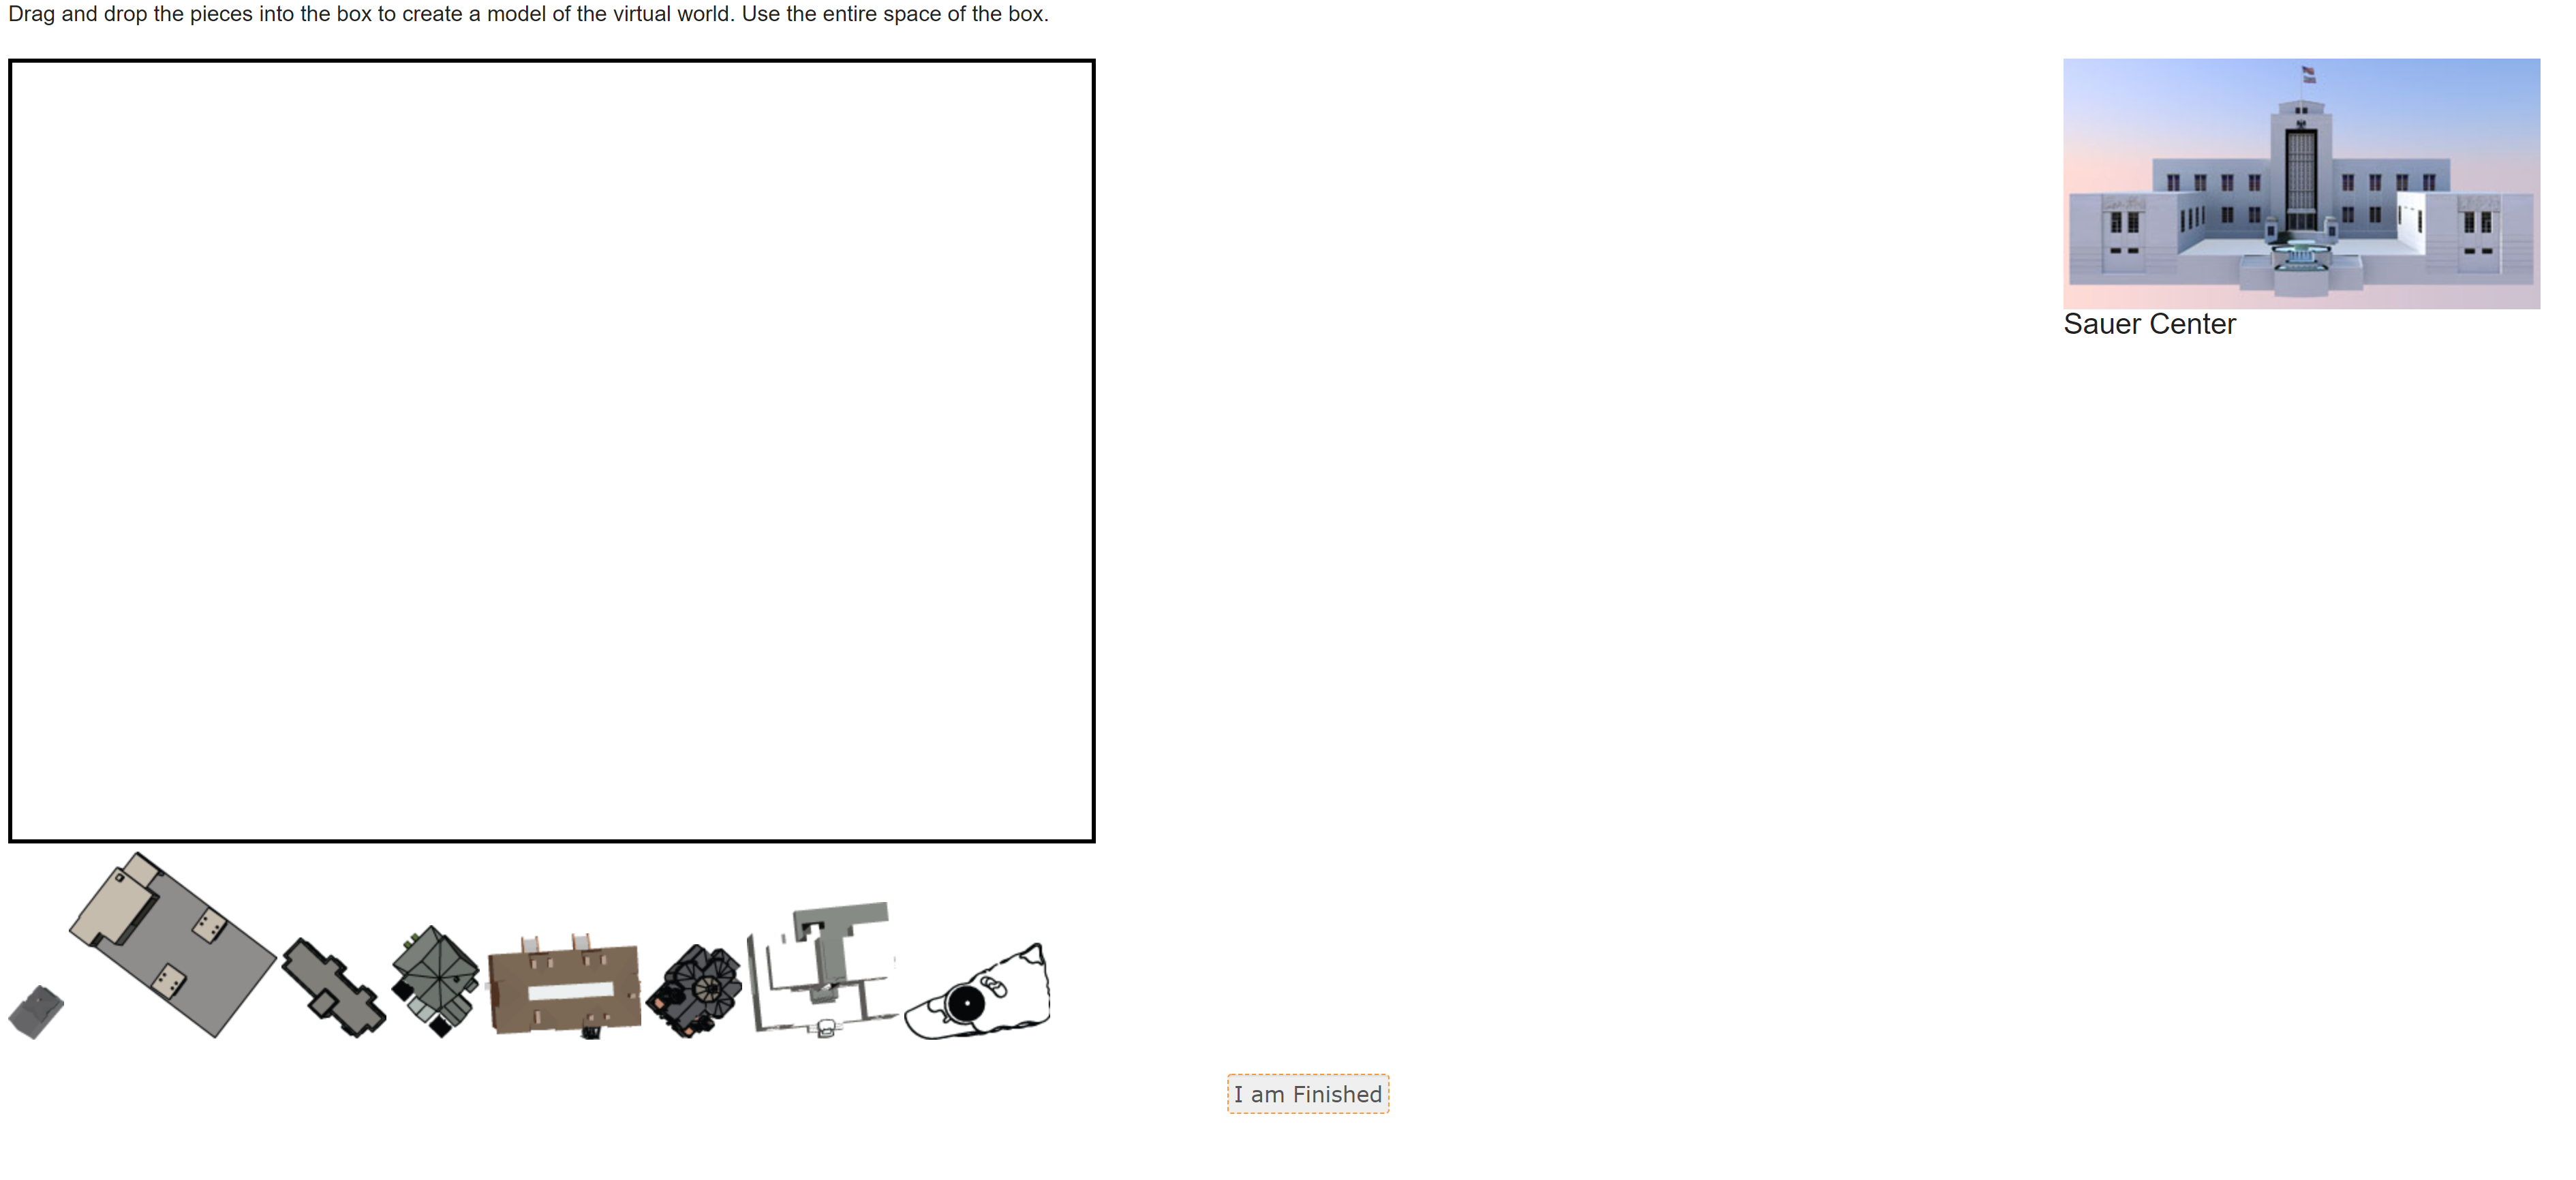
\includegraphics{./figs/Model_Building.png}
\caption{Virtual Silcton Onsite Pointing}
\end{figure}

\hypertarget{offsite-pointing-task}{%
\subsection{Offsite Pointing Task}\label{offsite-pointing-task}}

The logic of the offsite pointing task is the same as the Onsite Pointing Task. The Participant ``begins'' at each landmark, and indicates the directions to all other landmarks as if they are facing the next landmark. For example, in the image below, the Participant should imagine standing along the route next to Batty House, facing toward the gem (or diamond) indicating Lynch Station. The Participant must then drag and drop each of the grey rectangle to the position on the black circle that indicates the direction a compass needle would point if it pointed directly at the front door of that building. For example, if the Participant thought that the front door of Batty House was directly to her left, she should place the grey rectangle containing Batty House on the ``West'' position of the circle (or 9 o'clock).

Once all grey rectangles have positioned while at that ``location,'' the Participant clicks ``Next'' and the next location is loaded as a new circle.

Similar to the Model Building Task, hovering over the names of the buildings or diamonds provides a front view of the building.

\begin{figure}
\centering
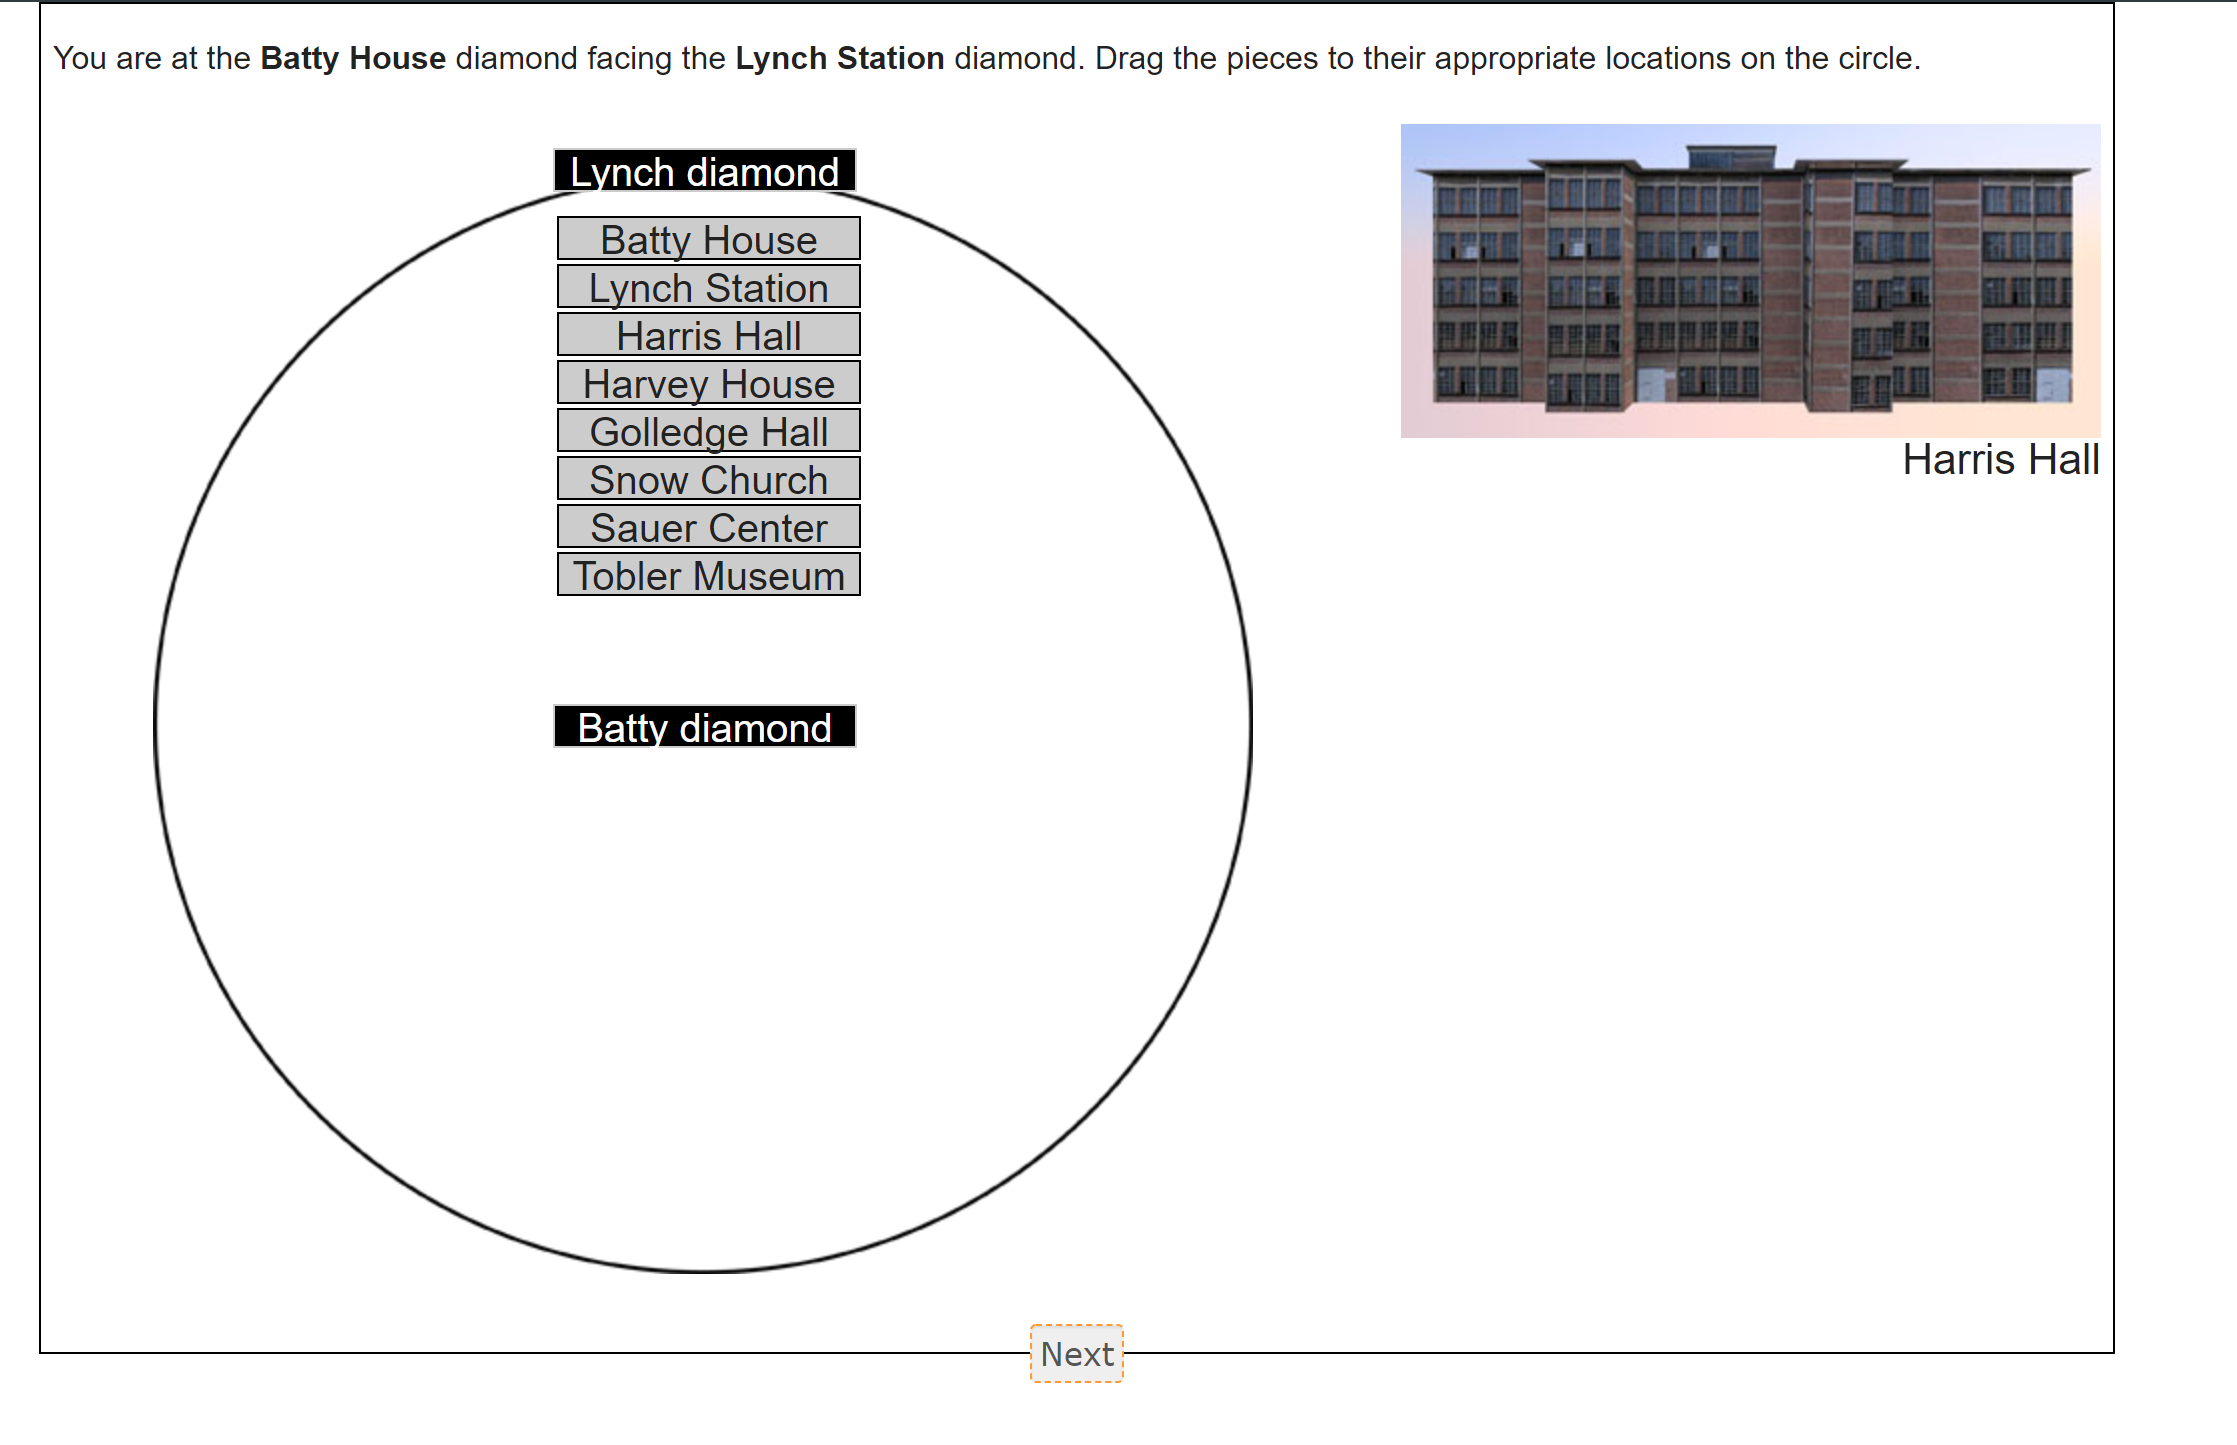
\includegraphics{./figs/Offsite_Pointing.png}
\caption{Virtual Silcton Offsite Pointing}
\end{figure}

\hypertarget{distance-estimation-task}{%
\subsection{Distance Estimation Task}\label{distance-estimation-task}}

The Distance Estimation Task requires the Participant to indicate the relative distances to and from each pair of landmarks. The Participant can view the distance from one landmark to another (in the figure below, the distance between Harris Hall and Batty House is set). The longest distance will always be the full length of the slider. The Participant must then set each other distance. Once all judgments have been made from one landmark (e.g., Harris Hall, below), clicking Next will load the next set of distance judgments with a new reference distance.

To my knowledge, data on this task has not been published, nor has it been validated with other measures. In my (SMW) experience, participants find it somewhat confusing. For that reason, we do not recommend it.

\begin{figure}
\centering
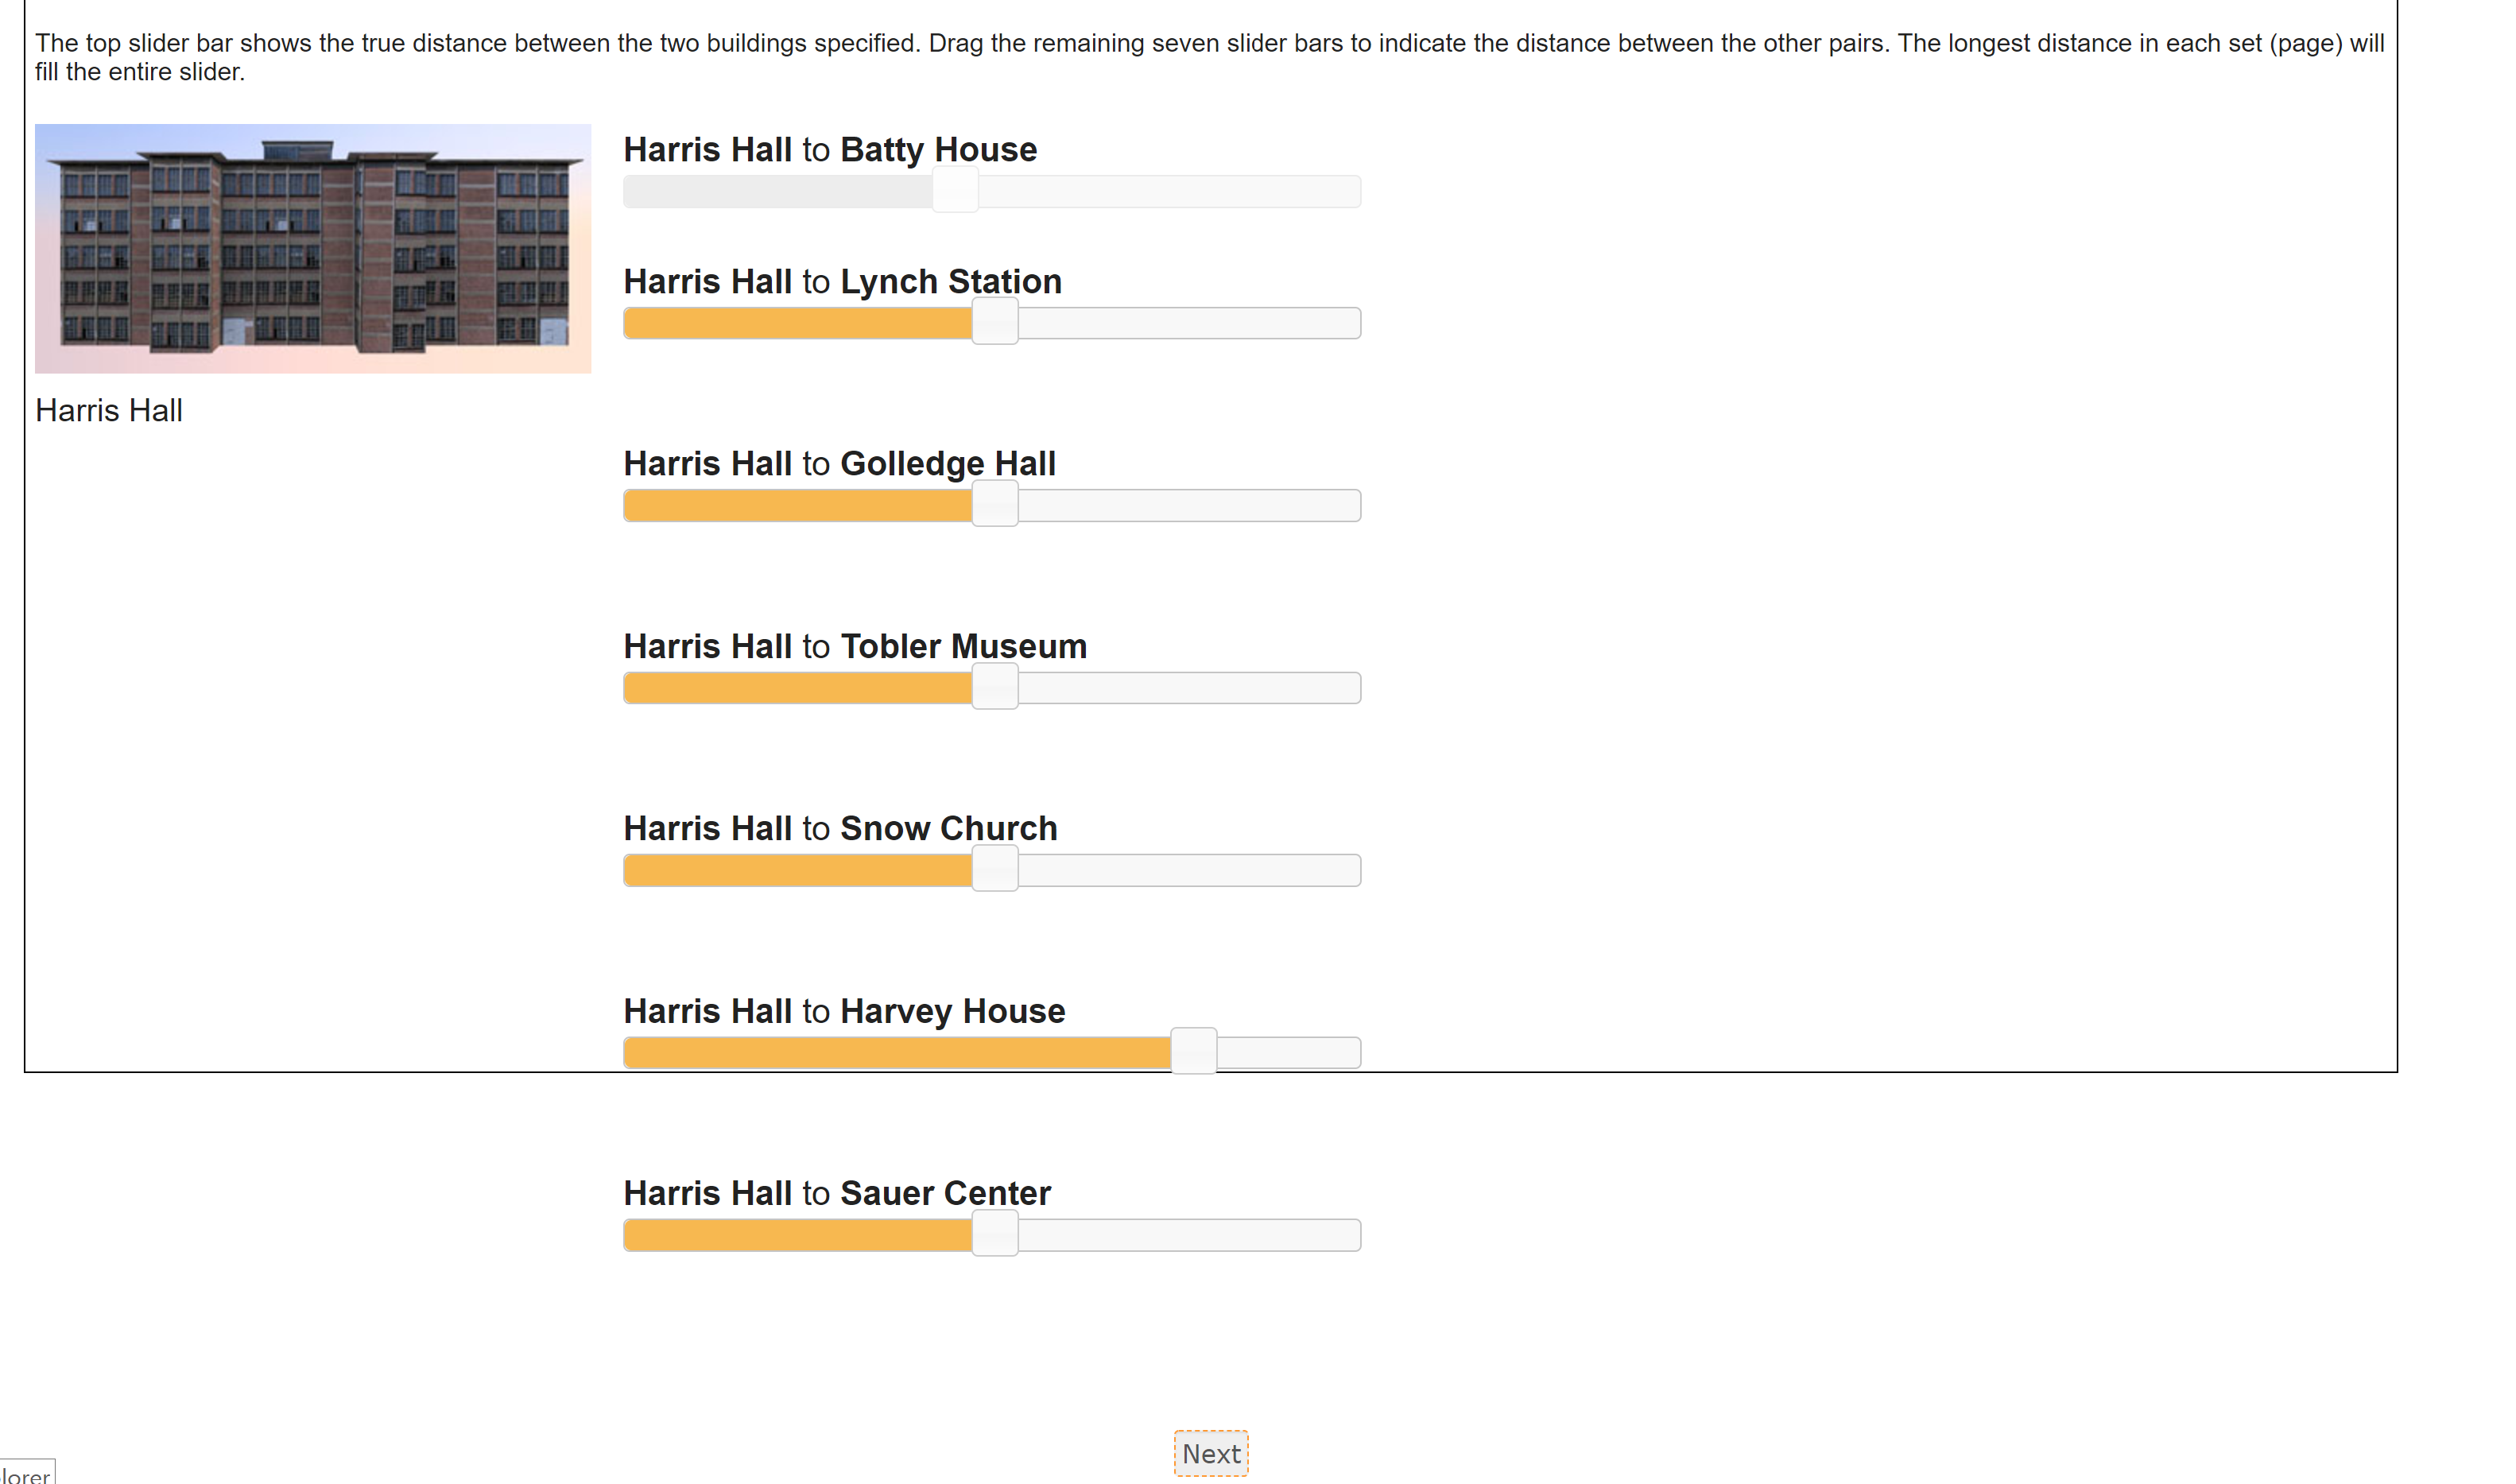
\includegraphics{./figs/Distance_Estimation.png}
\caption{Virtual Silcton Distance Estimation}
\end{figure}

\hypertarget{other-measure-descriptions}{%
\chapter{Other Measure Descriptions}\label{other-measure-descriptions}}

\hypertarget{introduction-page}{%
\section{Introduction Page}\label{introduction-page}}

At the beginning of each Study, two measures are automatically included: Informed Consent and Web Data Release.

At the top of the Intro Page, the Welcome Text appears, along with the name of the Study. Below that is the Participant's UUID and an option to select ``Pilot subject.''

The pilot subject checkbox is for experimenter internal use. If you wish to indicate that a Participant is just a Pilot Subject, indicate that by checking ``Pilot subject.'' The only thing this changes is how the Participant's data is labeled on the ``View Participants'' page.

\hypertarget{consent}{%
\subsection{Informed Consent}\label{consent}}

The consent form and web data release are automatically included in all studies.

Again, be advised, IRB approval and consent procedures MUST BE SEPARATELY ADMINISTERED at the home institution of the Silcton user.

In order to store data on our servers, the Participant MUST consent to allow anonymized data to be stored on the website. The version of the consent form that participants agree to on the website allows administrators to view the anonymized data. If the Participant does not consent, they can not be enrolled in the Study.

We require the following language to be included in any IRB protocol and informed consent involving Virtual Silcton:

\begin{quote}
An anonymous version of the data collected on the website from this study will be accessible to the
administrators of that website (Virtual Silcton). None of your personal, identifying, or confidential
data will be collected on this website.
\end{quote}

The Participant provides informed consent by clicking ``I Agree'' at the bottom of the Intro Study page.

\begin{figure}
\centering
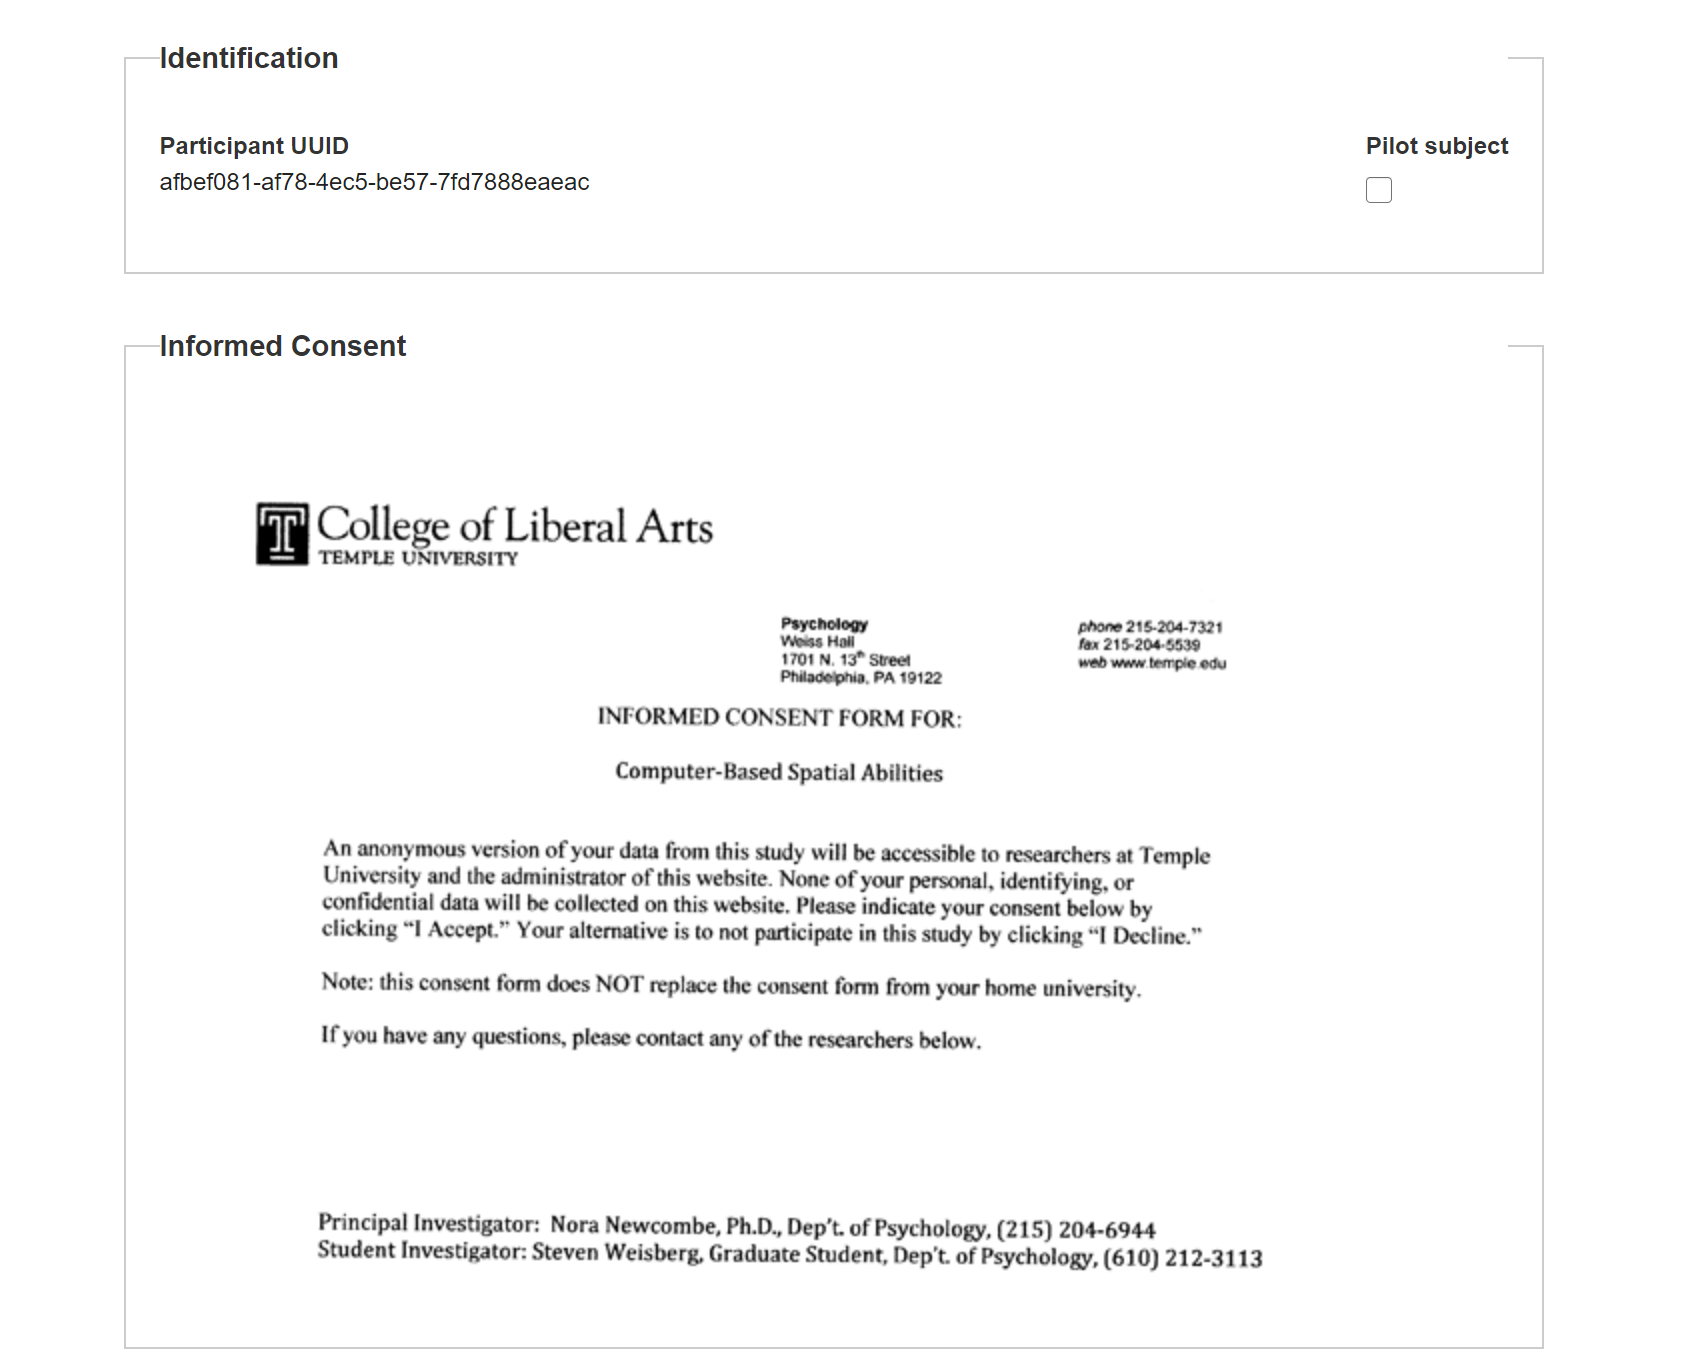
\includegraphics{./figs/Intro_Page_1.png}
\caption{Informed Consent on Intro Page}
\end{figure}

\hypertarget{web-data-release}{%
\subsection{Web Data Release}\label{web-data-release}}

The second automatic item (included in all studies) is the web data release form. This form allows the Participant to grant permission to share their anonymized data with any researchers who wish to access it and who are granted that ability by the adminstrators.

The web data release can be declined and the Participant can still take part in the Study. To agree to the web data release, the Participant selects `Yes' in the yellow box and enters their initials. (Initials are NOT stored on the website). To decline, the Participant selects `No.'

\begin{figure}
\centering
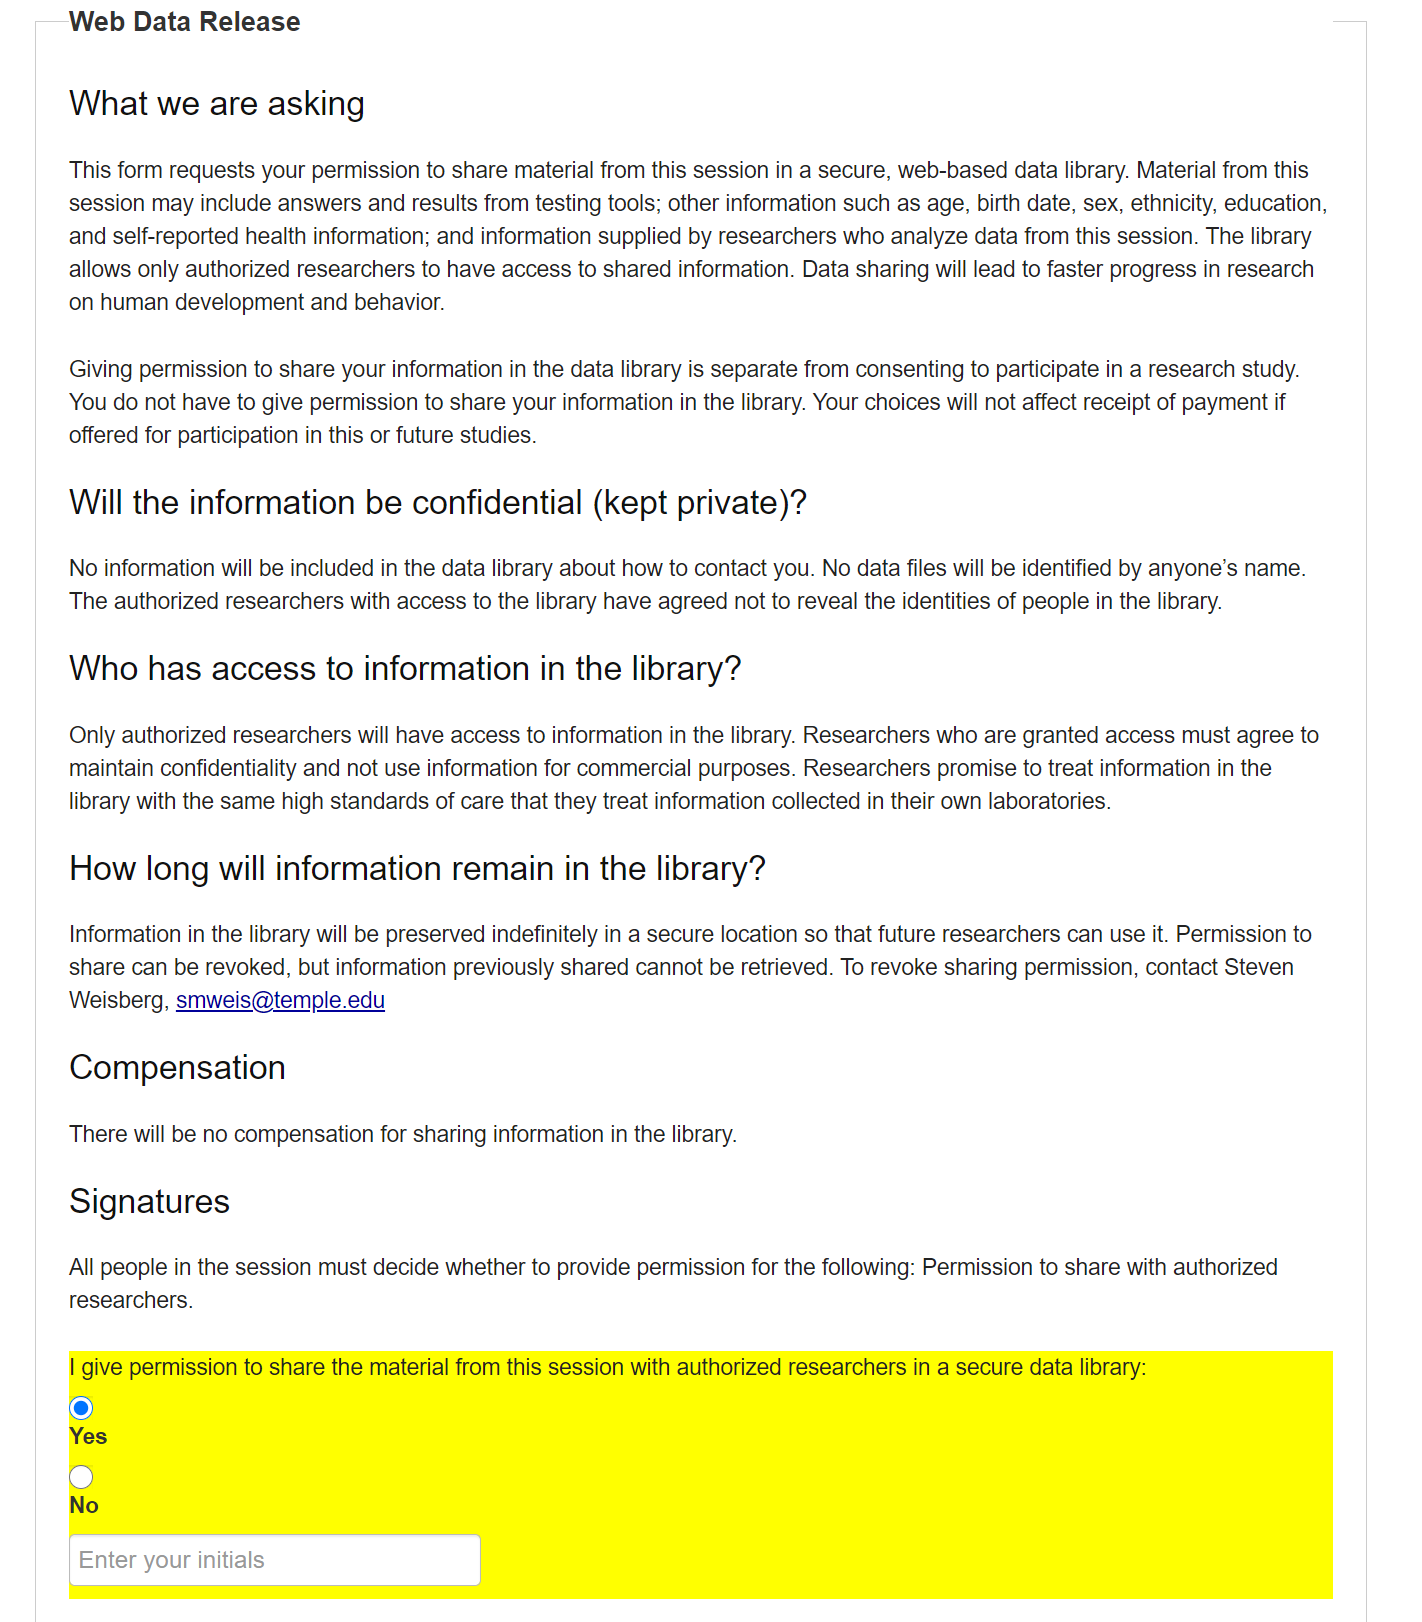
\includegraphics{./figs/Intro_Page_2.png}
\caption{Web data release}
\end{figure}

\hypertarget{demographics}{%
\section{Demographics}\label{demographics}}

Basic demographic information.

\hypertarget{santa-barbara-sense-of-direction-scale}{%
\section{Santa Barbara Sense of Direction Scale}\label{santa-barbara-sense-of-direction-scale}}

The SBSOD is a self-report measure of navigation ability. For more information, see \href{https://www.silc.northwestern.edu/santa-barbara-sense-of-direction-sbsod/}{here}.

\hypertarget{philadelphia-verbal-ability-scale}{%
\section{Philadelphia Verbal Ability Scale}\label{philadelphia-verbal-ability-scale}}

The PVAS is a self-report measure of verbal ability. More info \href{https://link.springer.com/chapter/10.1007/978-3-642-14749-4_10}{here.}

\hypertarget{philadelphia-spatial-ability-scale}{%
\section{Philadelphia Spatial Ability Scale}\label{philadelphia-spatial-ability-scale}}

The PSAS is a self-report measure of small-scale ability. More info \href{https://link.springer.com/chapter/10.1007/978-3-642-14749-4_10}{here.}

\hypertarget{mental-rotation-test}{%
\section{Mental Rotation Test}\label{mental-rotation-test}}

The MRT is an objective measure of small-scale spatial ability requiring participants to match a target figure to two rotated versions of the figure (and correctly reject two non-identical figures). As administered here, the MRT consists of sample problems, practice problems (which the participant must get correct), and two sets of 10 test items. Each set of test items is timed, the Participant has 3 minutes per set. Once time expires, that set will end. More info \href{https://www.silc.northwestern.edu/library-of-shepard-and-metzler-type-mental-rotation-stimuli/}{here.}

\hypertarget{updates}{%
\chapter{Updates}\label{updates}}

Two major updates are listed first. The rest will be listed in reverse chronological order once there have been updates.

\hypertarget{updates-to-the-pointing-task}{%
\section{Updates to the pointing task}\label{updates-to-the-pointing-task}}

In February 2020, a bug was brought to our attention affecting the standalone and website versions of the pointing tasks since we began using Virtual Silcton in 2010.

This bug was identified and fixed on both versions in May 2020. Data collected on the website is now identified on the website with a field for every pointing judgment that was affected (or potentially affected) by the issue.

Affected data: 2010 - May 2020
Effects of bug: Pointing judgments collected during this time were stored as absolute angles, rather than as signed angles. This bug had the effect of reducing the possible error range for certain pointing judgments (depending on a relatively arbitrary ``facing direction''). In sum, pointing judgments overall were scored with lower errors. This was the case for pointing judgments toward the building and away from the building. More details on the effects of this bug are forthcoming.

\hypertarget{updates-to-the-navigation-logs}{%
\section{Updates to the navigation logs}\label{updates-to-the-navigation-logs}}

In August 2020, we identified two irregularities with the navigation logs, which recorded facing direction and location (x,y) every .1 seconds. From when the navigation logs were instituted until May 2019, the logs only recorded the first \textasciitilde4 minutes. But the data were correctly recorded. From May 2019 until September 11, 2020 (for the main routes), the navigation logs recorded the absolute value of the facing direction rather than the facing direction itself (the quarternion, to be precise). It is therefore possible, but difficult, to reconstruct the actual facing direction in most cases. From September 2020 on, the navigation logs recorded correctly.

\hypertarget{part-analysis-and-scripts}{%
\part{Analysis and Scripts}\label{part-analysis-and-scripts}}

\hypertarget{data-analysis-tips-and-scripts}{%
\chapter{Data Analysis Tips and Scripts}\label{data-analysis-tips-and-scripts}}

The analysis github repository contains the available code for coding and analyzing some of the website data. Hopefully this capacity will be increased over time.

\hypertarget{onsite-pointing-data}{%
\section{Onsite Pointing data}\label{onsite-pointing-data}}

For canonical analyses, the onsite pointing data can be aggregated within participant and different/same route judgments.

\hypertarget{navigation-logs}{%
\section{Navigation Logs}\label{navigation-logs}}

Navigation log data are text files for each route the participant experienced.

These data have the following properties:

They begin 5 seconds into each route.
They record position and facing direction with the resolution of 10Hz.
Each position vector is: {[}x,y,z,theta{]}. y-values stay the same through the route because the participant does not move vertically.

Theta = 0 is a vector pointing ``Up'' on the Virtual Silcton map.

The corners of the map are defined with the coordinates:
Lower left: {[}-750, Y, -700{]}
Lower right: {[}700, Y, -700{]}
Upper left: {[}-750, Y, 300{]}
Upper right: {[}700, Y, 300{]}

\begin{figure}
\centering
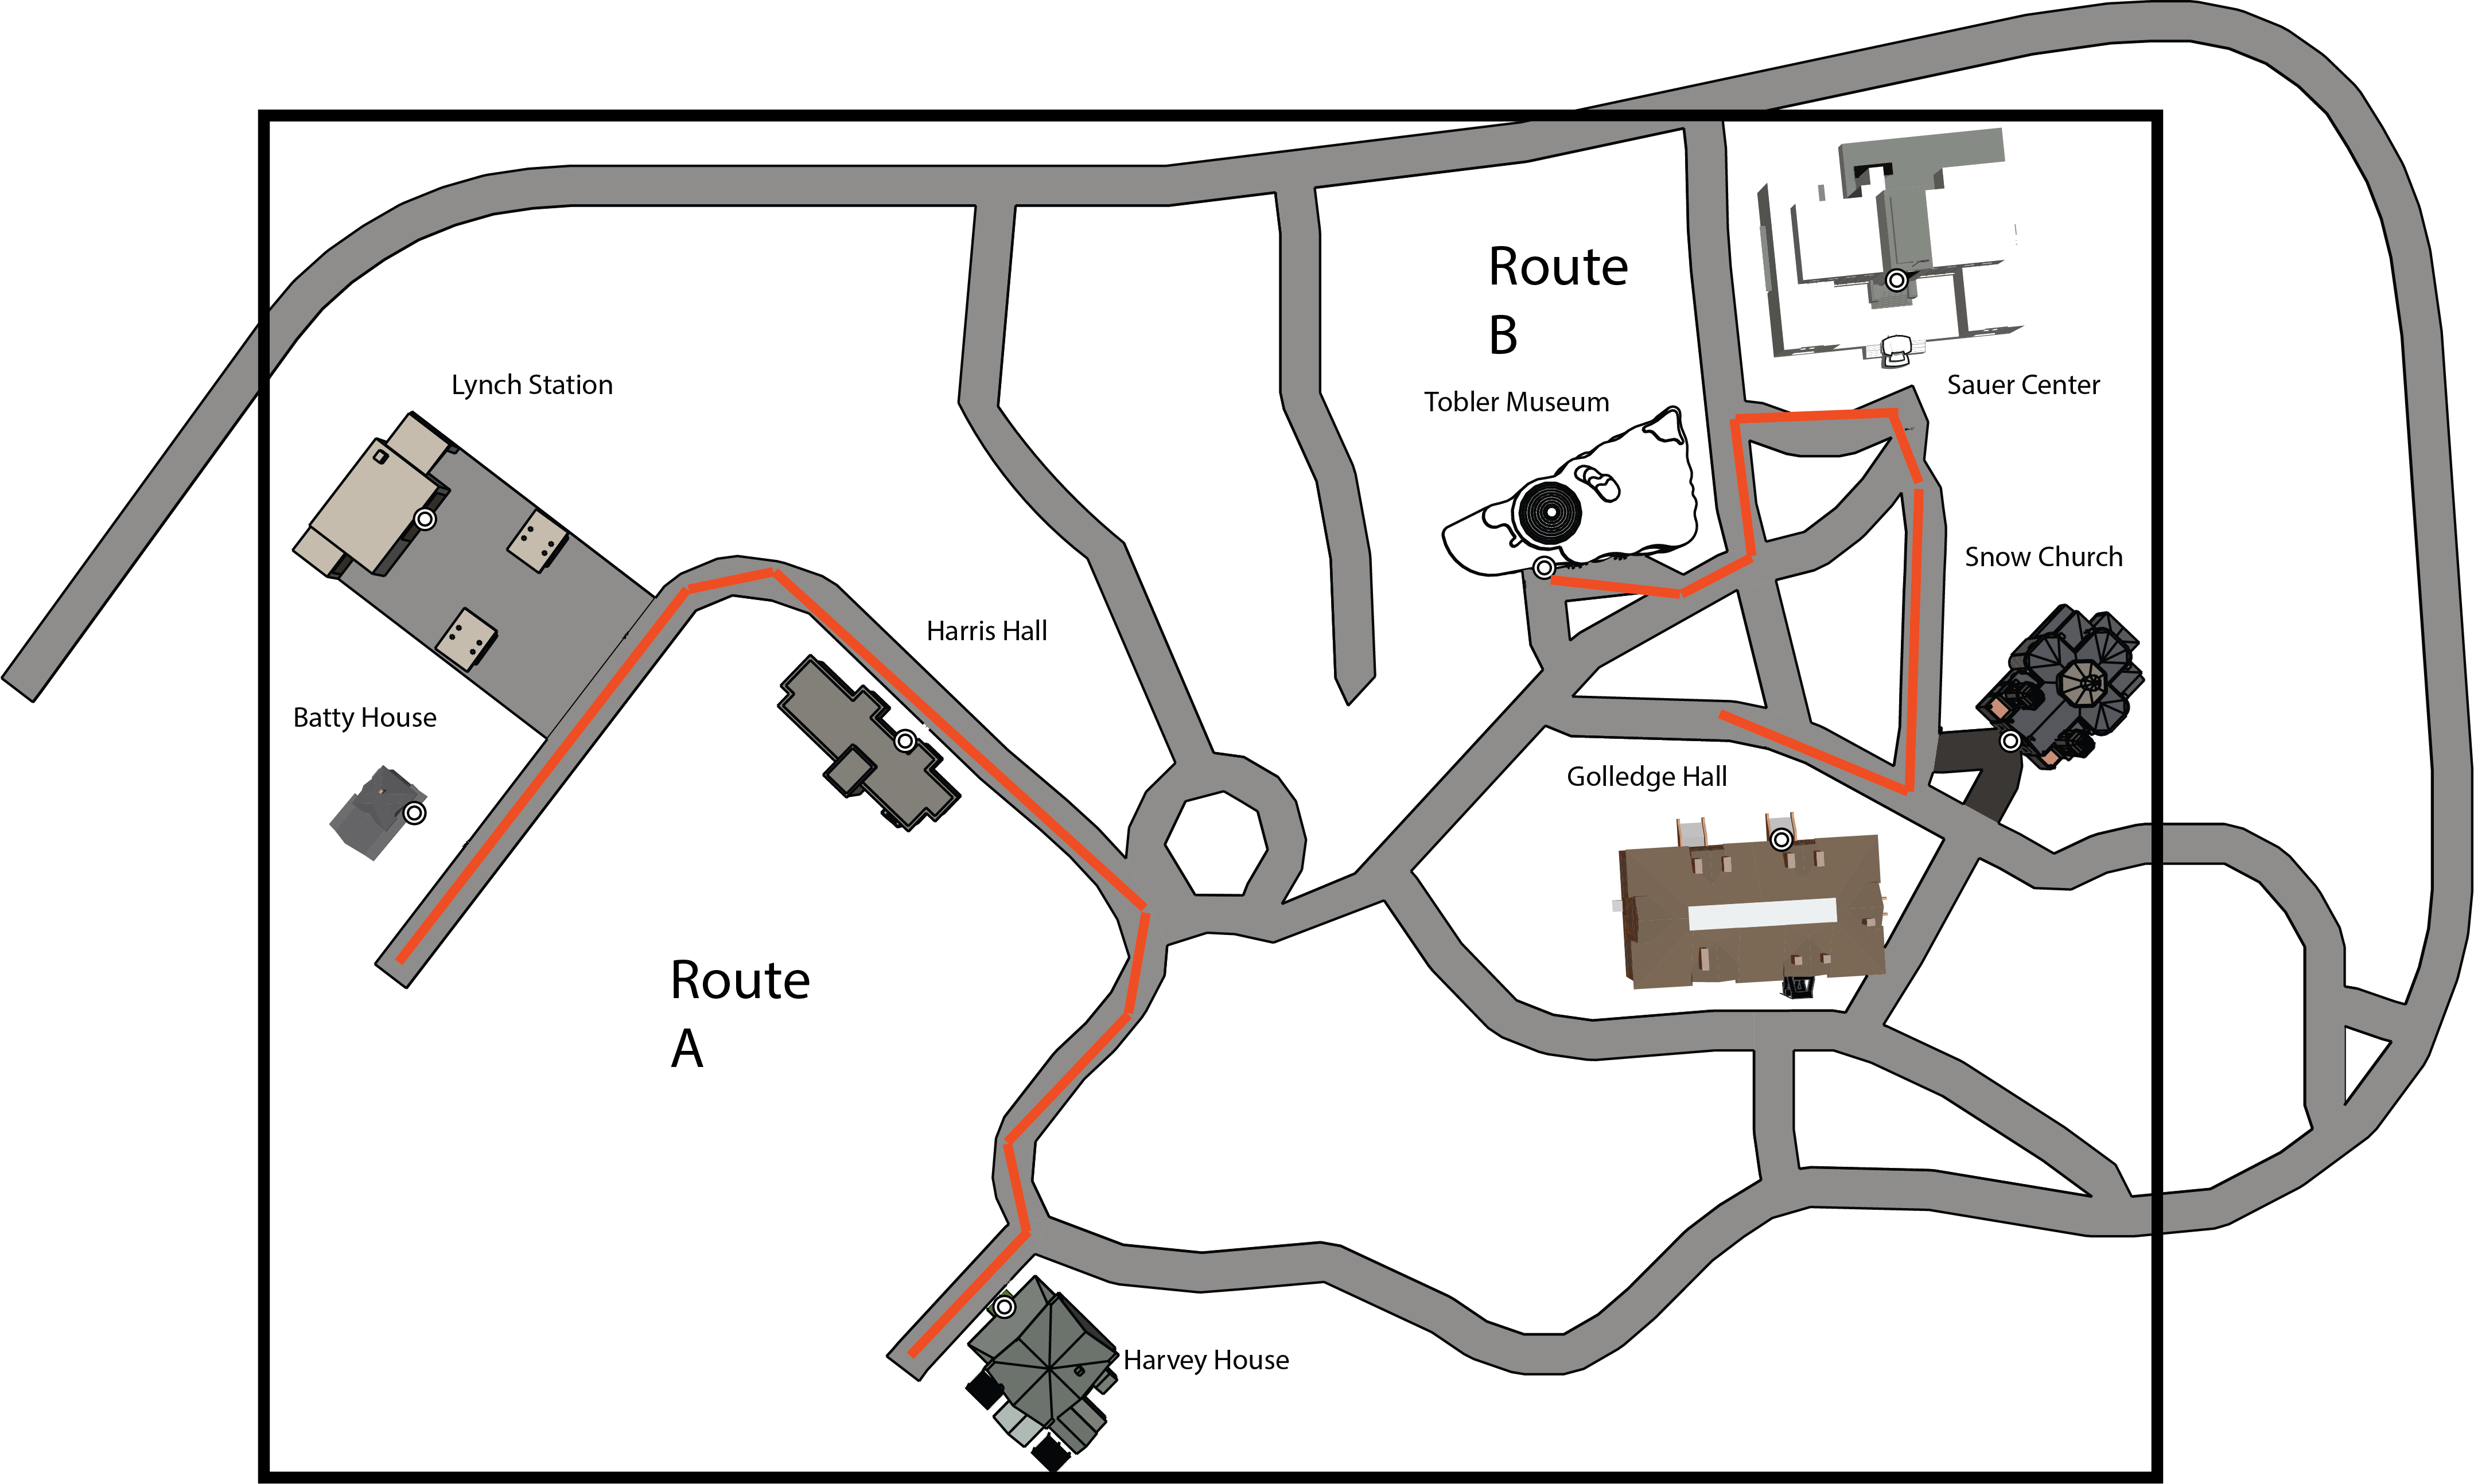
\includegraphics{./figs/Silcton_Map.png}
\caption{Virtual Silcton Map (Red lines highlight main routes)}
\end{figure}

\hypertarget{model-building-tasks}{%
\section{Model Building Tasks}\label{model-building-tasks}}

The model building task data can be downloaded and analyzed using the scripts found in the /ModelBuilding directory of the \href{https://github.com/smweis/Virtual_Silcton_Analysis}{Analysis git repo}

  \bibliography{book.bib,packages.bib}

\end{document}
